\documentclass[a4paper,11pt]{kth-mag}
\usepackage[T1]{fontenc}
\usepackage{textcomp}
\usepackage{lmodern}
\usepackage[latin1]{inputenc}
\usepackage[swedish,english]{babel}
\usepackage{modifications}
\usepackage{url}
\usepackage{csquotes}
\usepackage{graphicx}
\usepackage[colorinlistoftodos,prependcaption,textsize=tiny]{todonotes}
\title{Learning Playlist Representations for Automatic Playlist Generation}

\author{Erik Aalto}
\date{Juni 2015}
\blurb{Master's Thesis at Spotify and CSC\\KTH Supervisor: Carl Henrik Ek\\Company Supervisor: Boxun Zhang\\KTH Examiner: Danica Kragic}
\trita{TRITA xxx yyyy-nn}
\begin{document}
\frontmatter
\pagestyle{empty}
\removepagenumbers
\maketitle
\selectlanguage{english}
\begin{abstract}
  Spotify is currently the worlds leading music streaming service. As the leader in music streaming the task of providing listeners with music recommendations is vital for Spotify. Listening to playlists is a popular way of consuming music, but traditional recommender systems tend to focus on suggesting songs, albums or artists rather than providing consumers with playlists generated for their needs. This thesis presents a scalable and generalizeable approach to music recommendation that performs song selection for the problem of playlist generation. The approach selects tracks related to a playlist theme by finding the characterizing variance for a seed playlist and projects candidate songs into the corresponding subspace. Quantitative results shows that the model outperforms a baseline which is taking the full variance into account. By qualitative results the model is also shown to outperform professionally curated playlists in some cases.


\end{abstract}
\clearpage
\begin{foreignabstract}{swedish}
  Spotify \"{a}r v\"{a}rldens ledande service f\"{o}r musikstreaming. Som ledare inom musikstreaming \"{a}r musikrekommendation ett centralt omr{\aa}de f\"{o}r Spotify. Att lyssna p{\aa} spellistor \"{a}r ett popul\"{a}rt s\"{a}tt att konsumera musik, men traditionella system f\"{o}r musikrekommendation fokuserar snarare p{\aa} rekommendation av l{\aa}tar, album eller artister \"{a}n att tillhandah{\aa}lla spellistor genererade efter konsumenters behov. Denna avhandling presenterar en skalbar och generaliserbar metod f\"{o}r musikrekommendation f\"{o}r att v\"{a}lja l\"{a}mpliga l{\aa}tar f\"{o}r spellistegenerering. Metoden v\"{a}ljer l\"{a}mpliga l{\aa}tar genom att hitta den varians som karakteriserar den spellista man vill anv\"{a}nda som bas f\"{o}r generering och projicerar sedan kanididatl{\aa}tar ner i motsvarande delrymd. Kvantitativa resultat visar att modellen presterar b\"{a}ttre \"{a}n en referensmetod som anv\"{a}nder den fulla variansen. Kvalitativa resultat visar att modellen i vissa fall presterar b\"{a}ttre \"{a}n professionellt kurerade spellistor.

\end{foreignabstract}
\clearpage
\renewcommand{\abstractname}{Acknowledgements}
\begin{abstract}
 Writing this thesis I realize that I am a lucky guy. I have had the opportunity to work on a very interesting project, with engaged supervisors who have been there for me from start to end. Therefore I would like to start off with thanking my supervisors Carl Henrik Ek and Boxun Zhang. Thank you for having created the opportunity for me to write this thesis, for believing in me and for making this thesis a fun and learning experience. I have had a great time working with you. I further owe a great deal of gratitude to my fellow Spotify thesis workers Anders Pettersson and Matteo Poletti, thank you for all the good times and the interesting discussions. I want to thank Ahmad Qamar from Spotify New York, thank you so much for walking me through all the cool things that are happening with Machine Learning in NYC. I also want to thank the rest of Spotify for making this thesis a reality and a special thanks goes to the Analytics team, thank you for all the support.  Last, but definitely not least, I would like to thank my partner, Maria, for being supportive, understanding and always standing by my side, you are simply the best.
\end{abstract}
  

\clearpage
\tableofcontents*
\mainmatter
\pagestyle{newchap}
\chapter{Introduction}
This chapter intends  to provide the reader with an overview of the fields of music consumption and recommendation as well as the outline and limitations of this thesis project.

\section{Project Introduction}
Spotify is a music streaming service that provides music content from a very large database. As of the writing of this thesis the Spotify song library contained over 30 million songs with over twenty thousand songs added on a daily basis\cite{spotifyPress}. Spotify generates revenue by charging a fee from subscribing users, this service is called \textit{Spotify Premium}. A free version of music streaming is also available where revenue is obtained by presenting users with ads. Record companies, who own the music streamed from Spotify, are paid according to the popularity of the tracks for which they hold digital rights. Spotify was launched in October 2008 and today over twenty percent of the user pool subscribe to the premium service with over 15 million paying subscribers and over 60 million users in total\cite{spotifyPress}.

The consumption of music in the Spotify client can be done by listening to individual songs, top charts, albums, Spotify Radio or playlists created by either users themselves or professional playlist curators. The use of playlists is a popular means of consuming music and Spotify currently holds over 1.5 billion playlists, a number that is larger than the number of songs provided by Spotify by several magnitudes\cite{spotifyPress}. Playlists are particularly interesting in the context of music consumption as well curated playlists intend to create a specific atmosphere that can be enjoyed without interaction from the user. Albums can also be seen as playlists and when the iTunes store was launched controversies were caused as users were allowed to buy individual songs and thus loosing the particular experience album creators seeked to create. The importance of playlists can still be seen today as some songs only can be bought as part of an album on iTunes, without mentioning the numerous number of DJs who are striving for the creation of the perfect music experience for a specific moment. 
Given that a user has a preference for a specific playlist, an interesting feature would be to generate a playlist similar to the one a user has a preference for, but with different songs. This type of feature is interesting as it allows users to get music recommendations fitted to their needs. Such a feature could give Spotify a competitive edge in the hardening competition for music streaming customers and provide a complement to the manually curated playlists provided by Spotify.

The process of automatically suggesting music adapted to a specific user is a field of its own and is called recommendation. More specifically the software providing such recommendations are called recommender systems. Recommender systems provide an automated way to filter and rank information of interest for a certain user, possibly also taking time into account. A famous example of recommender systems is the product recommendation once initiated at Amazon, \textit{"Users who bought this product also bought"}. Another example of recommender systems are the movie recommendations provided by Netflix. Movie recommendations are interesting and non-trivial as a specific user at a certain time is likely to not be interested in the majority of movies provided by Netflix. The importance of good recommendations can be seen from the creation of the \textit{Netflix Prize}, a challenge created by Netflix to improve the movie recommendations provided by them. The Netflix Prize was a contest intending to improve the prediction of user ratings for unseen movies with a 1 million dollar premium for the winning team. A further example of recommendation could be restaurant recommendation, where time and context are important factors. Recommending a simple hamburger restaurant is not likely to be of interest at date night, but it might be the perfect recommendation while driving the kids home after Saturday morning soccer game. Recommender systems also exist within the music context, but typically consists of recommending individuals songs, albums or artists. Generating playlists that are suited for a specific theme, context time or task is something that today is missing within the Spotify client, despite listening to playlists is a popular way of consuming music.

\section{Project Aim}
The aim of this thesis is to provide a scalable method for selecting candidate songs, in the context of playlist generation, given a predefined playlist to mimic. This is an extension to the current work within music recommendation at Spotify.  

The work of this thesis is limited to finding candidate songs when generating playlists similar to seed playlists found within Spotify \textit{Browse}. The focus is on creating a scalable model of doing so. Focusing on the model means that features will be treated in an abstract way, just like abstraction layers within software engineering. Feature engineering will therefore not be treated. Likewise is the problem of ordering songs in playlist generation outside the scope of this thesis. 

\chapter{Background}

Previous work within the recommender system domain mainly focuses on two approaches. These are collaborative filtering and content based approaches. A hybrid of these two approaches can also be used. Both collaborative filtering and content based approaches typically try to infer a user ranking for a specific item\cite{melville2002content}. An item would in the context of music recommendation be a song, artist or album. This section will present these traditional approaches to recommendation. As these approaches do not focus on the playlist generation problem specifically work directly related to solve this task is also presented.

\section{Collaborative Filtering}
The goal of recommender systems based on collaborative filtering is to infer a user's ranking of previously unrated items and present the user with items corresponding to high inferred ratings. In a formalized way collaborative filtering can be said to present a user $u \in U$ with products $p \in P$ that the user has not yet rated such that the ratings $R_{up}$ for those products are maximized\cite{breese1998empirical}.

\begin{figure}
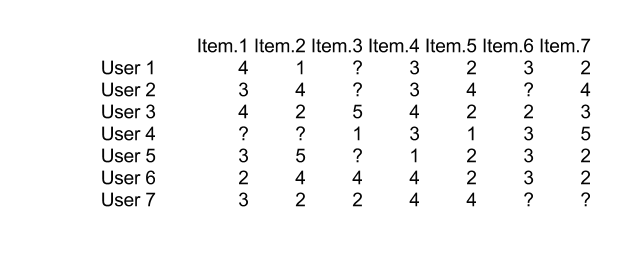
\includegraphics[scale=0.6]{images/colFiltMat.png}
\caption{Image illustrating the problem collaborative filtering intends to solve. The question marks are items that the specific user have not rated. Collaborative filtering intends to infer these ratings.}
\end{figure}

 Collaborative filtering focuses on user's past behaviour. From the past behaviour of a specific user and past behaviour of similar users the ranking for the specific user for a certain item is inferred\cite{sarwar2001item}\cite{su2009survey}. In other words, a user gets recommendations of items that other users with similar taste like\cite{adomavicius2005toward}. Finding similar users mean that some type of similarity metric must be used. Often items and users are mapped into vector spaces and distance metrics are used as similarity metrics. A distance metric could be the euclidean distance, but also the cosine value of the angle between vectors, also known as the cosine similarity or cosine distance, is used for collaborative filtering\cite{sarwar2001item}. 
 Collaborative filtering has the advantage that it typically relies on past user behaviour without the need of explicit user profiles\cite{melville2002content}. This means that only the past behaviour of a user is needed to use collaborative filtering.  As collaborative filtering, in the general case, only looks at user data it is also domain free, i.e. the model is not dependent on whether users have rated books, movies, music or a combination thereof\cite{hu2008collaborative}.

Collaborative filtering can be used with explicit user feedback. One example of explicit user feedback are the movie ratings used by Netflix or the thumbs up or thumbs down method used by the radio streaming feature from Spotify. Collaborative filtering can also be used with implicit user feedback\cite{hu2008collaborative}. In the music context implicit feedback could be whether a song has been played or skipped and in the movie context implicit feedback could be if a movie is watched for more than fifteen minutes or not.

Collaborative filtering methods can be divided into two categories, memory-based and model-based. Memory-based collaborative filtering algorithms can be seen as user based as they try to find recommendations based on what other users like. The model-based algorithms can be seen as item based, as they often seek to find similar items to the ones for which a user has a liking\cite{sarwar2001item}.

Memory-based collaborative filtering algorithms operate on the entire user-item matrix where the full user history data set is used\cite{breese1998empirical}. The user-item matrix could for example consist of one user per row and one item per column. This data set is used to predict a preference for a previously unseen item for a specific user. To perform predictions first the rows most similar to the row corresponding to the specific user are found. The ratings of the users corresponding to these rows for the unseen item are then used to predict the rating for the specific user. As similar user's ratings are used to predict a specific user's rating memory-based models can also be thought of as neighbourhood models as similar users are treated as the nearest neighbouring users in user space\cite{hu2008collaborative}. There are various ways of implementing a memory-based model, but a naive way could be to find similar rows by using the cosine similarity and then simply averaging the rating of the top-n similar users for a specific item. This naive approach has a $O(MN^2)$ complexity where M is the number of users and N the number of items. One downside of this approach is that it does not scale very well when the user-item matrix is large. Another downside is that the user-item matrix is likely to be very sparse. Imagine a online retailer that has millions of products, one percent of a million is ten thousand and a typical user is likely to have rated less than ten thousand products. Using a nearest neighbour approach in this sparse setting can lead to poor performance\cite{sarwar2001item}\cite{su2009survey}. The reason for this poor performance is that in a high-dimensional space the distance to the closest point, for any given point, approaches the distance of the furthest point as the dimensionality increases for many distributions\cite{beyer1999nearest}. This would mean that for a given user the inferred ratings for previously unseen items would have equal weights from users similar and different to the given user.

Model-based collaborative filtering means that the user history data is used to create a probabilistic model for ratings. At run time the model, rather than the entire user history data set, is used to make predictions of items for users\cite{breese1998empirical}. Model-based approaches are likely to scale better than memory-based ones\cite{sarwar2001item}. One approach to model-based collaborative filtering is to use latent factors. This means that each user would be associated with a user-factors vector $x_u \in R^f$ and each item with an item-factors vector $y_i \in R^f$. The predicted value of a user for an item would then be the inner product between the corresponding user and item vectors, i.e. $\hat{r}_{ui} = x_u^T y_i$. To avoid overfitting the model can be regularized, which means penalizing complex models. A cost function as follows is then obtained: 
\begin{equation}
min_{x_*,y_*} \sum (r_{ui} - x_u^Ty_i)^2 +  \lambda(||x_u||^2 + ||y_i||^2)
\label{corFilt1}
\end{equation}

In this equation the latter part is the added penalization, which can be seen to penalize large values for $x$ and $y$.

The problem with equation \ref{corFilt1} is that it assumes knowledge of explicit feedback. In the context of music recommendation the case is rather that implicit feedback is available than explicit. It is for example much easier to collect information about which songs a user has listened to than to collect ratings. Even if ratings are collected, then the number of songs a user has streamed is likely to be much larger than the number of rated songs.. What can be done in this case is to use binary labels expressing whether a user has preference for an item or not. Having preference for an item could mean that the user has streamed that song and not skipped it for example. Therefore the binary variable $p_{ui}$ is used to describe user preference.

There is however an uncertainty to the preference a user has. Has a user really preference for a song that is selected on Spotify Radio while the user was in another room? What can be done is to create confidence variables, that could depend on the number of times a song has been streamed. What can be done here is to use another variable \[ c_{ui} = 1 + \alpha r_{ui} \] where $r_{ui}$ is the number of times user \textit{u} has streamed item \textit{i}. The $\alpha$ term is to weight the number of times a song has been streamed.

The resulting cost function then becomes:
\begin{equation}
min_{x_*,y_*} \sum c_{ui}(p_{ui} - x_u^Ty_i)^2 +  \lambda(||x_u||^2 + ||y_i||^2)
\end{equation}

Problems still remain as users and items can contain bias. The remedy is to enter bias terms, the resulting cost function is then:

\begin{equation}
min_{x_*,y_*} \sum c_{ui}(p_{ui} - x_u^Ty_i - b_u - b_i)^2 +  \lambda(||x_u||^2 + ||y_i||^2)
\end{equation}

Where $b_u$ is the user bias term and $b_i$ is the item bias term.

The resulting problem is a non-convex optimization problem, but by fixing either the user or item vectors the problem becomes convex and can be solved by the use of alternating least squares, where the cost function is guaranteed to get a lower value with each iteration\cite{hu2008collaborative}. This approach is similar to the collaborative filtering method used used in production at Spotify.

The downside with collaborative filtering is that it suffers from something called the cold start problem or first rater problem. If a user yet have not rated any items collaborative filtering will fail to give that user good recommendations. The same things applies to items that no one has yet rated, if items have not been rated neither can they be recommended\cite{herlocker2004evaluating}\cite{melville2002content}. In the context of Spotify where twenty thousand songs are added each day this will pose a problem.

\section{Content Based Approaches}
In contrast to collaborative filtering approaches content based recommendation suggest items that are similar to items  a user has had preference for in the past. This can be done by either comparing items to items or to create a user profile based on a users preferred items\cite{adomavicius2005toward}. Content based recommendation requires a representation of each item and or user, typically by mapping items and users into vector spaces. An rudimentary example of user profiles created from preferred items would be to represent a user by an initially empty vector and each time the user presents preference for an item the item vector is added to the user vector which is then normalized. Content based approaches look at discrete features of items and tries to infer a similarity between two items given their similarity of features. Similar to the approach of finding similar users in memory-based collaborative filtering distance metrics can be used as similarity measures in content based recommendation. A parallel can be drawn between content based recommendation and information retrieval. In the context of content based recommendation the utility function that is maximized is the similarity between items, which typically is the inverse of the items distance\cite{adomavicius2005toward}. One of the main features of content based recommenders are that they are able to provide recommendations even when little user history data is available, something that is one of the major drawbacks of collaborative filtering\cite{gunawardana2009unified}.

Different approaches can be used to create the features used in content based recommendation in the music domain. One approach is to simply have human experts annotating tracks with information\cite{musicGenome}\cite{tzanetakis2002musical}. Other approaches could be to extract properties from the audio signal. One such example is the use of MFCCs, which creates features from short time intervals of each track\cite{logan2000mel} and another is to use Deep Belief Networks\cite{hamel2010learning}.

An interesting property of content based recommendation is that it allows for relevance feedback, for example with use of the Rocchio algorithm. The Rocchio algorithm allows for a user to select a subset of recommended items as relevant and move the recommendations displayed towards the direction of those items in the vector space items are represented in\cite{pazzani2007content}.

Downsides with content based recommendation are that a user can never be recommended something that is not similar to what the user has expressed preferences before in the past. Further, content based recommendation is limited to the features of items. If the features used to describe items are poor a content based recommender system is likely to perform poorly. Lastly, content based recommenders do not take sequential information into account. Thus a well written news article is seen identical to the same article written backwards as they contain exactly the same words\cite{adomavicius2005toward}.

\section{Hybrid Systems}
Hybrid systems are recommenders that combine both the techniques of collaborative filering and content based filtering, with the purpose of thus obtaining better recommendations. The underlying assumption is that a combination of content based recommenders and recommenders using collaborative filtering can redeem the weaknesses these methods face on their own\cite{gunawardana2009unified}. 

Hybrid recommenders can be made by combining the results of collaborative filering methods with content based methods, by incorporating properties of one method into the other or by creating a model that incorporates properties of both types of systems\cite{adomavicius2005toward}. 

A simple example of a hybrid system could be create an ensemble model that weight scores from content based and collaborative filtering based recommenders. Given an item $i \in I$ that has an inferred rating $r_collaborative filtering$ from a collaborative filtering recommender and an inferred rating $r_content based$ from a content based recommender a way of combining thesis approaches could be to simple set the rating of the hybrid model to \[ r_{hybrid} = \alpha_1 r_{collaborative filtering} + \alpha_2 r_{content based}\] Here $\alpha_1$ and $\alpha_2$ are the weights to each of the individual recommenders.

One way of combining collaborative filtering and content based recommendation into one single method is to first create user ratings for all items that are completely lacking ratings by a content based method. For example, for all users that rated a product similar to the unrated item a content inferred rating can be created by taking a user's rating of the item closest to the unrated item and multiplying it with one minus the cosine similarity of the items $r_{unrated}  = (1 - (cos(i_{rated},i_{unrated})) * r_{rated})$. This matrix can then be used for traditional collaborative filtering and the cold start problem for unrated products will no longer be an issue. Another way of tackling the same problem would be to infer ratings of all unrated items for all users in a similar manner and then use collaborative filtering to weight the vote of each previously unrated item for a specific user. An approach that have been used to find improvement in recommendation over a pure content based approach\cite{melville2002content}.
\section{Playlist Generation}
The approaches of recommendation presented gave a general overview to the field of recommender systems. However, these approaches where either based on item to item recommendation or recommendations of the type item to user. The problem this thesis intends to solve regards music or more specifically playlists, why previous work related to playlist generation is presented here. 

\subsection{Probabilistic Graphical Models for Playlist Generation}
Earlier attempts of playlist generation has been made by Microsoft Research\cite{ragno2005inferring}. Ragno, Burges and Herley has made a model for playlist generation that employs probabilistic graphical models. Probabilistic graphical models can be said to be graph-based models that give a compact way of describing the structure in a distribution. A probabilistic graphical model describes the conditional dependence between random variables in the form of a graph\cite{koller2009probabilistic}. In a music setting this could mean that given that a song A is spotted in a playlist we can get the probability for song B being in the same playlist. The probabilistic graphical model used for playlist generation by Ragno, Burges and Herley can take any type of ordered playlist material, such as curated playlists or albums, as training data, and use this input data to generate playlists as output data. The initial step in the model is to create an undirected graph. 

\begin{figure}
\centering
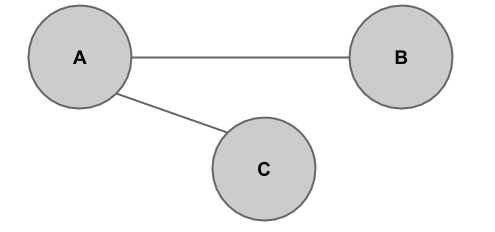
\includegraphics[scale=0.4]{images/UGM.png}
\caption{Illustration of an undirected graph. Here transitions between nodes A and B can be made, transitions can also be made between nodes A and C. No direct transitions between nodes B and C can be made.}
\end{figure}

In this graph each song will be represented by a node. Each edge in the graph corresponds to a first to nth ordered Markov property. What this means is that for a first order Markov property edges between songs adjacent to each other in a playlist or album will be present in the graph. For a second order Markov property songs that are one or two steps before or behind any given songs will have edges between the corresponding nodes. The weights corresponding to the edges in the graphs depends on how many times the songs fulfills the nth order Markov property in the input data. For example, if a song A is adjacent to a song B twenty times in the input data playlists the weights on the edge between node A and B will be twenty.

  Once the undirected graph is created for all songs in the music library a directed graph is created from the undirected graph.
  
\begin{figure}
\centering
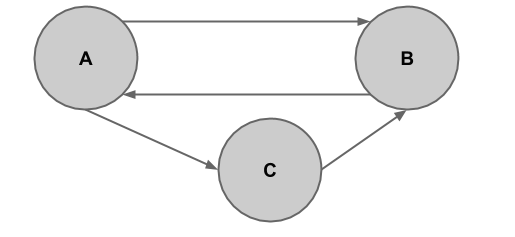
\includegraphics[scale=0.4]{images/DGM.png}
\caption{Illustration of a directed graph. Each edge corresponds to a one way transition. In this graph transitions can be made between nodes A and B both ways, transitions can be made one way from node A to node C but not from C to A. From node C transitions to node B can be made, but no transitions from node B to node A are possible.}
\end{figure}  
  
  When the undirected graph is converted into a directed graph the weights of edges, the transition probabilities, are normalized by the sum of outgoing weights from each node. That is if the edge between nodes A and B in the graph has a value of five and node B has outgoing edges which sum to ten and node A has outgoing edges that sum to fiften then the value of the directed edge from A to be will be $edge_{AB} = 5 / 10$ and the edge between B and A will have a value of $edge_{BA} = 5 / 15$. Once the directed graph is created a playlist can be generated by selecting an initial seed song, choosing a node as starting point, and simply performing a random walk in the graph. This model assumes that the connectivity between songs is independent of the order in input data. From one perspective this is a bad assumption as DJs, playlist curators and artists spend a large amount of time perfecting the order of songs, information that is lost in this model. On the other hand, consider the following example: song A is followed by song B five thousand times in input data, but song B is never followed by song A in. Then songs B and C both follow each other five times each. First creating an undirected graph and then a directed graph would not rank the connectivity between B and C as being higher, which is a reasonable behaviour. Lastly, a problem that might occur is something called playlist drifting. Playlist drifting would mean that the generated playlist would consists of songs in the following order: A, B, C, D. Where each song is realted to the song before, but song D might be completely unrelated to song A. The solution to this problem would be to use higher order Markov properties, that is adding taking songs further away from each song into considerationwhen creating the graphical model\cite{ragno2005inferring}. 

Problems with the directed graphical model approach taken to playlist generation by Rango, Burges and Herley is that if you generate a playlist from a random walk you cannot chose the playlist theme for the generated playlist on before hand. Another problem with the probabilistic graphical model approach to playlist generation is that the graph created during training phase only works for songs that are in the training data set. This model is not generalizable in the sense that as new songs are added updates are needed for the graph in which the random walk is performed to create a playlist. This is not an ideal situation for Spotify as a high quantity of songs are added to the Spotify music library every day\cite{spotifyPress}.


\subsection{Gaussian Processes for Playlist Generation}
An approach for playlist generation that is generalizable to data outside the data used to train the model is to employ the use of gaussian processes\cite{platt2001learning}. A gaussian process is characterized by its mean and covariance functions\cite{mackay1998introduction}. A gaussian process is a model that associates each data point with a stochastic normally distributed variable and provides a joint gaussian distribution over the data\cite{rasmussen2004gaussian}. Gaussian processes are useful when the number of dimensions is large compared to the number of data points. The setting of few data point but many dimensions is relevant in the playlist generation case. A playlist can be about ten, twenty or thirty songs long, while the number of dimensions for each song can be on the magnitude of music genres. As there are hundreds of music genres, the number of features for each song in a playlist might then very well exceed the number of songs in that playlist.  A gaussian process does not provide a direct function that reflects the data but rather a distribution over functions\cite{rasmussen2006gaussian}. To employ a gaussian process a prior assumption of distribution is needed and as data is seen the prior is updated according to data. This new distribution that incorporates data is called a posterior distribution. The posterior can then be used similarly as the prior for the next data point, then called the predictive posterior. 

In the work taken by Platt et al, also at Microsoft Research the authors try to learn a gaussian process prior from training data\cite{platt2001learning}. This prior is then used together with a set of songs, for which a user has expressed preference, to generate a playlist given an initial seed song. In the training phase a blend of linear kernels is used to learn the relationship of meta data features among songs that come in sequence. A blend of linear kernels is the same things as weighting several linear predictions where weights are learned from data. The coefficients for each linear kernel is learned by finding the coefficient that minimizes the difference between the empirical covariance between songs and the value given by the linear kernel. Empirical covariance is in this case as simple as whether the training data songs belong to the same album or not. Once the training phase is done the playlist generation phase consists of predicting the user preference for each song in a set of candidate songs. This is equal to calculating the posterior probability $p(preference For New Song | known Preferences)$. This probability is calculated by weighing the blend of linear kernels between a seed song and each candidate song with a factor. This factor is the sum of similarity between the initial seed song and each user preference song weighted by how central each user preference song is in the preference space. Playlist generation is then done by simply choosing the songs with highest probability for user preference\cite{platt2001learning}.

This model generalizes to new songs, but the user preference space is seen as one single space. This is a simplification of reality where a user preference space is probably divided into several categories, for example a workout preference space and a chill-out preference space, something the model provided does not take into account, which can be claimed as a weakness in terms of generating a playlist adapted for a specific theme or context. Neither does the model take the ordering of songs into account, but the authors argue that the ordering obtained from listing the songs by their predicted user preference value creates a good order of songs\cite{platt2001learning}.

\chapter{Representation Learning}
A popular way of music consumption is listening to playlists. Traditional recommender systems are not focused on creating playlists suited for a user, theme or moment. The goal of traditional music recommendation is rather recommendation of items given a certain user. What is then a reasonable approach to extend recommendation into the playlist context? If one starts with looking at playlists it is evident that playlists consist of songs as a playlist is a flow of songs. A random sample of songs does not make as good a flow of music as a carefully mixed playlist. One can therefore conclude that there is a relation between the tracks in playlists. The tracks in a playlist, even though being correlated, vary somehow. A good way of approaching the playlist generation problem then seems to be to learn how a playlists vary. Methods to learn the underlying factors of how a good playlist vary all involve learning a representation. Once a representation of a playlist is learned the representation can be used for playlist generation. This chapter will give an introduction to the field called representation learning and relate it to the generation of playlists.

\section{Representation Learning}
Representation learning is about learning the factors that represent something. The idea behind representation learning is that the data used for a task often can be represented in a simpler way that is more suited for the task at hand\cite{bengio2013representation}. This idea is nothing novel, even as far back as during the time of Greek rationalists and atomists the idea that observed data was dependent upon something latent was present\cite{mulaik1987brief}. Representation learning assumes that there is an intrinsic representation of data that is less complex than the observed representation. One example could be an image represented by pixels. If the image is of size 320 x 320 pixels it can be thought reasonable to assume that the image has an equivalent amount of degrees of freedom as pixels. However in an image of a man wearing a shirt every pixel is not independent as most shirt pixels are adjacent to other shirt pixels and thus not independent for example. As all number of pixels in an image do not vary independently of each other learning a representation of images also means that the number of factors learned are less than the number of pixels for each image in the data set. A lower number of learned factors than observed ones implies that a dimensionality reduction is made while learning a representation. 

Another explanation of learning representations is the one of Factor Analysis, which intends to describe how a number of observed variables vary together. One example could be points on a two dimensional plane in a three dimensional space. The points on the plane covary, but only in two dimensions. Therefore a dimensionality reduction can be made to describe the points in this plane, as they need not be described by three dimensions. However we cannot be sure that the points only vary in lets say the \textit{x} or \textit{y} direction. The directions in which the points vary must be learned and does not have to be well represented in the original dimensions of the vector space. These two learned dimensions of the plane then becomes the latent factors of the representation.
Factor Analysis can be used in an exploratory way as a means of learning the underlying factors of something we want to represent, but it can also be used to synthetically generate data once the latent factors of the original data are learned.

\section{Principal Component Analysis} 
Learning a representation is about extracting latent factors from connected data. Connected data means that the data points in the data set examined are related to other data points in the same set. As there is covariance in the data latent factors can be learned. One way of deriving latent factors due to linear relationships in the data is Principal Component Analysis, PCA. What PCA can be said to do is to connect the covariance in a data set to a set of principal components that explain the variance in the data. Another explanation to PCA is that it models the variance in the data into principal components that are ranked depending on how much of the variance in the data they explain. To provide a better understanding of PCA  lets look at its derivation:

\begin{equation}
C \in R^{D x D}
X \in R^{N x D} 
C = (X - \mu)^T (X - \mu)
argmin_A {||C - A||}_F = \left\{C = V \lambda V^T = \sum_{i=1}^{D}\lambda_i v_i v_i^T \right\} 
\end{equation}

\begin{equation}
= \left\{ A = \sum_{i=1}^{D}\gamma_i v_i v_i^T \right\} = {|| \sum_{i=1}^{D}\lambda_i v_i v_i^T - \sum_{i=1}^{D}\gamma_i  v_i v_i^T ||}_F = {|| \sum_{i=1}^{D}(\lambda_i - \gamma_i) v_i v_i^T ||}_F 
\end{equation}

\begin{equation}
= {|| \sum_{i=1}^{d}(\lambda_i - \gamma_i) v_i v_i^T + \sum_{i = d}^{D}\lambda_i v_i v_i^T ||}_F
\end{equation}

Here \textit{X} is our data and \textit{C} is the covariance matrix of the data observed. A is an approximation of the covariance C and as can be seen from the derivation above. A approximates C up to a certain threshold of variance, if the full variance is covered then A will equal C, but if C only goes up to a certain threshold of variance a dimensionality reduction is made. In the general setting this means that a high threshold of variance, for example 90 percent, can be explained by $d < D$ dimensions. These dimensions that explain the major part of variance in the data can also be seen as the latent factors of the data. These factors are linear combinations of the original dimensions of data and are orthogonal to each other. Doing Principal Component Analysis of a data set is the same as doing an eigen decomposition of the covariance matrix of the data and selecting eigen vectors corresponding to eigen values up to a certain threshold. As PCA takes a covariance matrix as input and gives latent factors as output PCA can be said to connect the covariance of the data to a representation of the data.

\begin{figure}
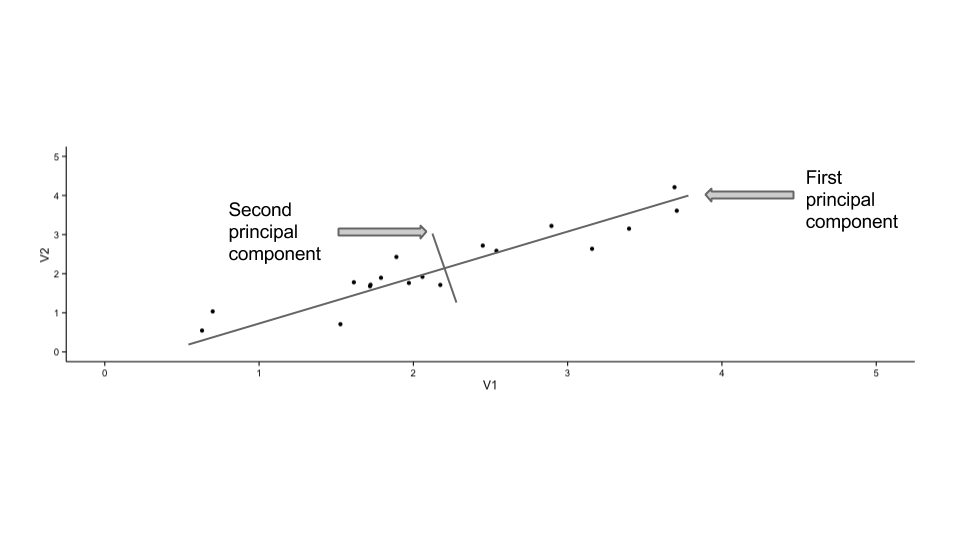
\includegraphics[scale=0.42]{images/pca.png}
\caption{Graphical illustration of PCA}
\end{figure}


As can be seen in the figure above, the first principal component lays in the direction that describes the largest part of variance in data. The principal components are orthogonal to each other. 

\chapter{Representing Playlists}
\begin{displayquote}
\textit{Without assumptions you cannot do machine learning} \\\\Ryan Adams
\end{displayquote}

This thesis intends to make an initial step towards fully automated playlist generation in the form of candidate song selection. The problem this thesis is trying to solve is to select a number of songs given a predefined playlist so that the selected songs constitute a playlist similar to the predefined one. This chapter will bring the reader through the process of investigating playlist data to the creation of representations with the help of that data. The reader will  be presented with some of the difficulties along the process and how playlist represenations are related to the problem of candidate track selection. Lastly theoretical shortcomings of the way a representation is related to the selection of appropriate tracks will be discussed. The remedy taken to compensate for the shortcomings will also be covered, together with the positive side effects this remedy brings along.

\section{Assumptions}
The goal of the thesis is to generate playlists, similar to seed playlists choosen by the user. In order to do this there is a need for assumptions regarding playlists.

\begin{itemize}


\item The first assumption for this thesis is that curated playlists, playlists made by professionals whose work is to create good playlists, suited for a specific context,genre or mood are suitable training data to create a model that generates playlists suited to the same playlist theme.

\item The second assumption made is that features that belong to each track in a curated playlist contain enough information to create a representation of the theme this curated playlist is made for.

\item The third assumption is that a playlist can be looked at as a good mixture of songs, i.e. there is an inherit variance in the playlist that defines it. This is a clear distinction from assuming that playlists only consist of songs similar to each other.

\end{itemize}
 

\section{Data}
To be able to learn representations of playlists there is a need for data. A classical notion within the machine learning community can densely be presented by the following quote by Bob Mercer \textit{"There is no data like more data"}. Recent studies however doubt this notion and currently a diversion towards less but better data can be spotted. An example is a study presented by Rehbein and Ruppenhofer where they show that passing the information that is needed to learn a task rather than flooding a model with data yields good results\cite{rehbein2010there}. As stated in the assumptions section in this chapter an underlying assumption is that playlists made by professional playlist curators provide a suitable base for learning playlist representations. Due to this assumption all playlists available from Spotify where not used, but the playlists used were limited to the ones created by professional playlist maker, so called playlist curators. Data for the tracks in these playlists were provided from Spotify including features consisting of discrete values for genre, mood and tempo for each track.

An important note regarding features is that they do not pertain within the scope or focus of the thesis. The scope of the thesis is rather to represent these features. The way this distinction affects the work of this thesis is that features are treated as a different abstraction layer than the focus of this study. Just like the driver of a car does not need to know how a car engine works to drive a car, this model treat feature data in a similar manner. Once someone has learned how to drive the car used is to a high degree irrelevant. In the same way this thesis seeks to investigate how representations of playlist data can be learned, without being tightly coupled to the data used to represent the tracks in playlists. At the same time, just as a driver can driver faster with a better engine, better feature data would also make the model presented work better.

\section{Exploratory Data Analysis}
The data set consisting of feature data for playlist tracks contains information and a good way of providing insight of information is visualization. In order to get an overview of how features in the data set relate to each other visualizations where made. A good way of visualizing relations in data is to plot covariances, in the context of playlist representation visualizing playlist feature covariances is therefore a reasonable approach. The approach taken was however to visualize correlations rather than covariances. The idea behind visualizing correlations instead of covariances is that the magnitude of the correlation shows the strength of the linear relationship between features, while a covariance plot would be polluted should different features be on different ranges. By plotting correlations the problem of calculating correlations for features with zero variance, given a seed playlist, emerged. Zero variance terms are a problem in the correlation setting as calculating the correlation for a zero variance term would imply dividing by zero, a mathematically undefined operation. This problem was solved by setting the correlation for feature relations with zero covariance to zero. It can be argued whether this is mathematically correct or not. But the approach can be motivated in this setting by the fact that plots are done to get an intuition of the data. A correlation of zero for features with zero covariance thus gives a better intuition of relationships in the data set compared to setting the correlation to one.

Performing visualizations of feature covariances in a playlist also shows whether there are linear realtionships among features in that playlist or not.

\begin{figure}
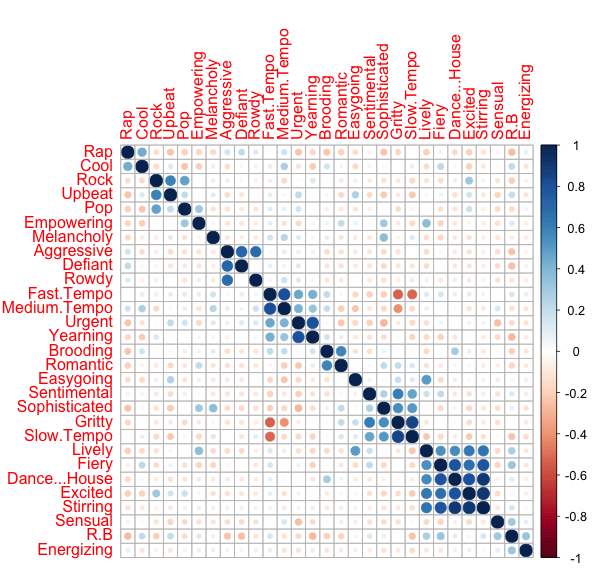
\includegraphics[scale=0.6]{images/0removedPlistFeaturePlot.png}
\caption{Visualization of covariances in a sample playlist. Zero variance terms have been removed. As can be seen there are linear correlations between features in the playlist data for this particular playlist. The conclusion that can be drawn from this is that there are dependencies between features and that the presence of certain features is related to other features and vice versa. This information is an important factor for modeling the characteristics of the playlist. The symmetry along the diagonal of the figure is due to relationships between features being two way. As can be seen from the geometry in the figure, features that are related are grouped into squares along the diagonal of the image.}

\label{plistCorrs}

\end{figure}


As we can see from \ref{plistCorrs}, there are clearly linear correlations among features for our example playlist. As relationships is shown to be prevalent in the data, these relationships can be learned and used to generate data similar to the data used as a base for learning these relationships.

\section{Learning Playlist Characteristics}
Once that linear relationships have been spotted in the data the next step is to create a model that can learn the representation of a specific playlist. One simple approach to learning latent factors in data is principle components analysis, PCA.
Explaining the characteristics for a certain playlist could be seen as equivalent of explaining the variance of features for tracks, given a curated playlist. Therefore extracting the main characteristics for a playlist can be done by extracting the principal components for the curated playlist. It is reasonable to assume that all the variance that is modelled by PCA is not of interest to model a playlist. Why PCA is performed up to a certain threshold for the variance explained, which means that the variance of interest is kept. By keeping the relevant variance a dimensionality reduction is made. The relevant variance is different for each playlist
Using this approach extracting eigenvectors for the covariance matrix, rather than correlation matrix, is a motivated choice. The motivation behind this choice is that scaling the covariance matrix to a correlation matrix is a nonlinear transformation. If we want to use apply the principal components of a correlation matrix to the original data, then the original data need to undergo the same transform as transforming covariances to correlations. For a data set where each curated playlist makes up less than one percent of the total data it would be impractical to transform the original data over and over as we extract the principal components for each playlist. Doing so would also not be feasible in terms of scalability. Using the covariance matrix for extraction of features is therefore motivated as the principal components of the covariance matrix can be directly related to the existing data.

\subsection{Handling zero variance terms}
Even though there are no zero variance terms in the whole data set, there are some terms that have zero variance within a certain curated playlists. These terms will not be handled by the principal components describing a playlist, as principal components describe the variance of a playlist. Despite not being handled by the principal components zero variance terms might still have an important role in describing a playlist. For example, if we have a curated jazz playlist then it is probably an important factor that all of the tracks in this playlist have a zero value for rap. The importance of this can be easily understood by imagining the opposite, what if those tracks would have a constant non-zero value for rap? Then a non-zero value for rap associated with jazz would be an important indicator for that playlist, why the absence must also be an important indicator.

\section{Selecting candidate songs for a playlist}
The process of selecting candidate songs given a specific seed playlist is a challenging problem without a given approach. Earlier work is focused mainly on item to item recommendation, i.e. recommending similar items of the same type given preferences for items of a certain times. But when it comes to selecting appropriate songs in the context of mimicing a playlist the items are of different kinds. The goal is to recommend songs, one type of item, given a seed playlist, which is another type of item. 

One initial idea to select songs for a given playlist could be that songs are either good candidates or not. This is a reasonable assumption, as for example for a rock classics playlist then songs are either rock classics or not. Given that this can be formulated as a binary classification problem, an efficient two class classifier might seem as a good idea at a glance. A support vector machine, SVM,  is an optimal two class classifier by definition, as a SVM maximizes the margin between classes\cite{cortes1995support}, and has the capability of multi class classification with for example the one versus all approach\cite{hsu2002comparison}. There is however one problem with support vector machines, or any classifier that requires training data within playlist generation. The problem is that it is easy to define training data which labels a song as belonging or not belonging to a certain playlist. But it is hard to define what songs that belong to other playlists, than the one describing a specific playlist theme, which are still relevant for that playlist theme. For example a song belonging to a house workout playlist may very well be a suitable candidate for a house party playlist. It is actually often the case that many songs belong to several playlists, describing different playlist themes. Given this example a discriminative model turns out to be a bad fit for the problem this thesis is trying to solve. If a song belongs to a house party playlist then it is reasonable to assume that it would be outside the margin defining a house workout playlist if feeded to a SVM, even though this particular song might very well be a suitable match for the house workout playlist. This rules out the use of SVMs for the purpose of this thesis, as SVMs need to know the mapping between songs and playlist themes to work. The same mapping that we are trying to find.

A second idea to selecting songs suitable for a specific playlist theme would be to use centroid based clustering. The wikipedia definition of clustering is as follows: "clustering is the task of grouping a set of objects in such a way that objects in the same group (called a cluster) are more similar (in some sense or another) to each other than to those in other groups (clusters)". One could for example cluster all tracks in curated playlists and then simply assign each song that is not part of a curated playlist to the cluster providing the best fit for each track. But one problem is that there is not a one to one mapping between tracks and playlists, one playlist can contain many tracks and one track can belong to many playlists. This is different from clustering where each cluster consists of many points, but each point only belongs to one cluster, which yields centroid based clustering impropriate for the scope of this thesis. 

A third approach to finding candidate songs given a playlist theme would be to tweak the normal usage of collaborative filtering. The common approach of collaborative filtering is to use a sparse matrix to infer the rating of items for one user given the ratings of similar users. What can be done instead is to use binary ratings and instead of inferring ratings for a user one could infer ratings for songs given a playlist. What this means is that playlists that contain the same songs as a playlist describing a playlist context one is interested in will be used to infer songs that are good matches for the specified playlist context. 

\begin{comment}
Discuss collaborative filtering and content based approaches.
\end{comment}

\subsection{Subspace method}
Another approach for track candidate selection would be to use the subspace method. Given that the principal components for a playlist, are at hand, one can simply treat each track as a vector rather than a point. Each vector can then be projected into the principal component space for that playlist. The underlying assumption is then that points that have a low relative change in magnitude under projection are well described by the characteristics defining the playlist, and thus good candidates. Tracks that are not well described by the playlist characteristics on the other hand, will change under projection and will therefore also have a high relative change in magnitude. As all tracks will be projected this is actually a ranking algorithm where tracks with lower relative change in magnitude will have a higher rank and tracks with higher change in magnitude a lower rank. To illustrate how the subspace method works lets look at the following picture:

\begin{figure}
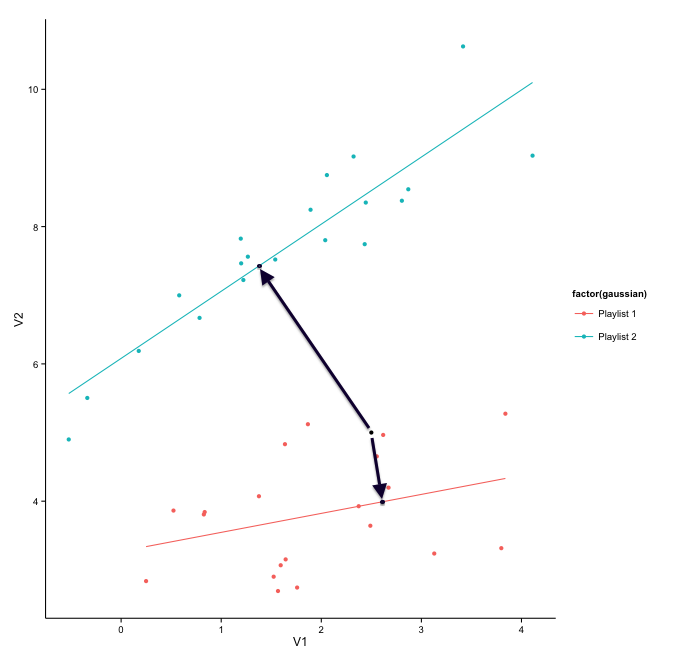
\includegraphics[scale=0.6]{images/subspaceIllustrationBW0.png}
\caption{Illustration of how points relate to principal component space under projection of the subspace method.}
\end{figure}


Here two playlists are illustrated in the two dimensional plane and their first principle component is the line through the points. As can be seen projecting the point into the principal component space of plaaylist 1 means a lower change of magnitude for the point than projecting the point into the principal component space of playlist 2. This means that the point, representing a track, provides a better fit for playlist 1 than playlist 2.

There are however problems with the subspace method. Lets say that there is a playlist that is defined by variance in the dimensions jazz, blues and rap and our vector space consists of the dimensions jazz, blues, rap and rock. If there is a song that is characterized by jazz and blues only, then this song will go unchanged under projection. As the relative change in magnitude is none then this song will be suggested as a suitable candidate for the jazz, blues, rap playlist. However a playlist consisting of variance in the dimensions of jazz, blues and rap is likely to be pretty peculiar and a song characterized by jazz and blues only is not likely to be a suitable match for such a playlist. Another problem would be songs that consists of zero values for all features, these songs would also go unchanged under any playlist principal component space projection, but are not likely to be good candidates for all playlist. Also if by looking at the definition of covariance 
\begin{equation}
\sigma(X, Y) = E[(X - E[X]) (Y - E[Y])^T]
\end{equation} 
one sees that covariance only takes the relative difference into consideration. That is if the variance of a variable is on the scale of five to twenty or from twenty to thirty five the direction of variance when applying the Principal Component Analysis will be the same. Therefore one can say that the subspace method only takes direction but not location into consideration as the use of covariance is a normalizing method.

Further, the subspace method is a linear transformation and it can be questioned if a linear transformation is powerful enough to describe the necessary mappings.

\section{Playlist Comparison}
As principal components were chosen to describe playlists, it is reasonable to assume that if principal components analysis works well for describing playlist characteristics, then the same approach should also work well for comparing playlists. Playlists were compared pairwise. To compare two playlists all eigenvectors from each playlist were multiplied by each other. If we think of playlist A as  \[A = U_1 \lambda_1 U_1^T\] and of antother playlist B as \[B = U_2 \lambda_2 U_2^T\] then the operation performed to compare them can be seen as \[M = U_1 U_2^T\] where M is the resulting matrix from the comparison. By doing this a measure proportional to the cosine measure of vector similarity for each pair of vectors was obtained. 

The problem with this approach is that it gives an unbalanced comparison. By simply looking at the similarity of eigenvectors implies that eigenvectors corresponding to low eigenvalues have the same importance as eigenvectors corresponding to high eigenvalues. This means that components explaining a high part of the characteristics of a playlist are regarded an equal importance as components explaining a low part of playlist characteristics. To remedy this problem the cosine score between eigenvectors from each playlist was scaled by the square root of the product of the corresponding eigenvalues, which mathematically can be formulated as  \[M = U_1 \sqrt{\lambda_1} \sqrt{\lambda_2} U_2^T \] The result obtained from this multiplication was a square matrix. To rank the similarity between these matrices some type of transformation from a matrix to a scalar is needed. The initial idea was to aggregate the entries of the matrix, but an aggregated value does not tell which values that have led up to the aggregated result. Therefore by simple adding values of the matrix one would not know if the similarity comes from dot products between vectors corresponding to high or low eigenvalues. The variance that is deemed as relevant is the one corresponding to high eigenvalues and the irrelevant variance the one corresponding to low eigenvalues. Therefore it was chosen to only take the matrix diagonal, the trace of the matrix, into consideration. Three different approaches were taken: the sum of the values of the diagonal, the absolute value of the sum of the diagonal and the sum of the absolute values of the matrix diagonal. These approaches were taken to compare 28 playlists among themselves.

\begin{figure}
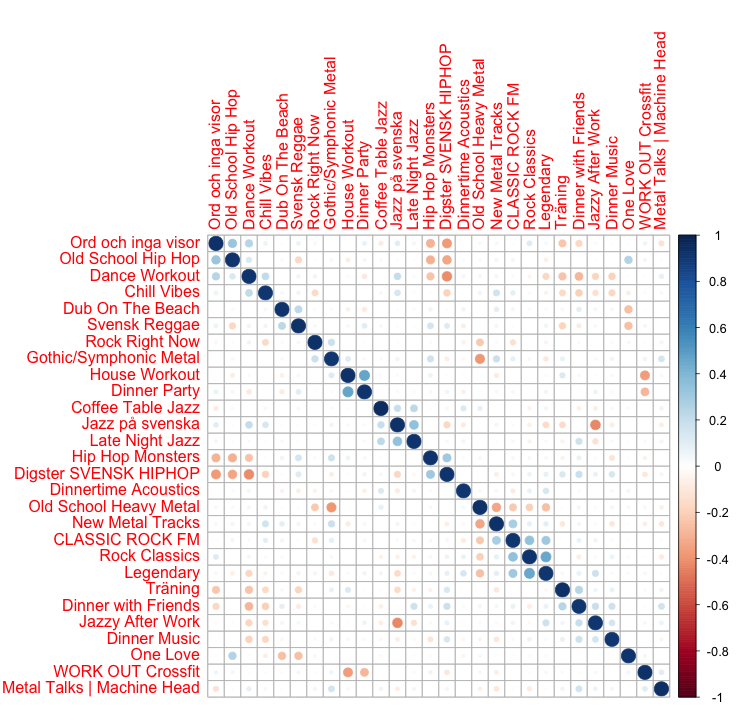
\includegraphics[scale=0.5]{images/sum.png}
\caption{Hierarchical clustering of playlists where the aggregated measure of the weighted dot product matrix is taken by the sum of the matrix diagonal. If one looks closely at the diagonal it can be seen that this approach clusters playlists together, in the form of squares around the diagonal. Clusters are mostly in a pairwise manner and are sensible. For example \textit{Dub on The Breach} and \textit{Svensk Reggae} are clustered together, as are \textit{House Workout} and \textit{Dinner Party}, as well as \textit{Coffee Table Jazz}, \textit{Jazz på Svenska} and \textit{Late night Jazz}.}
\label{sum}
\end{figure}

\begin{figure}
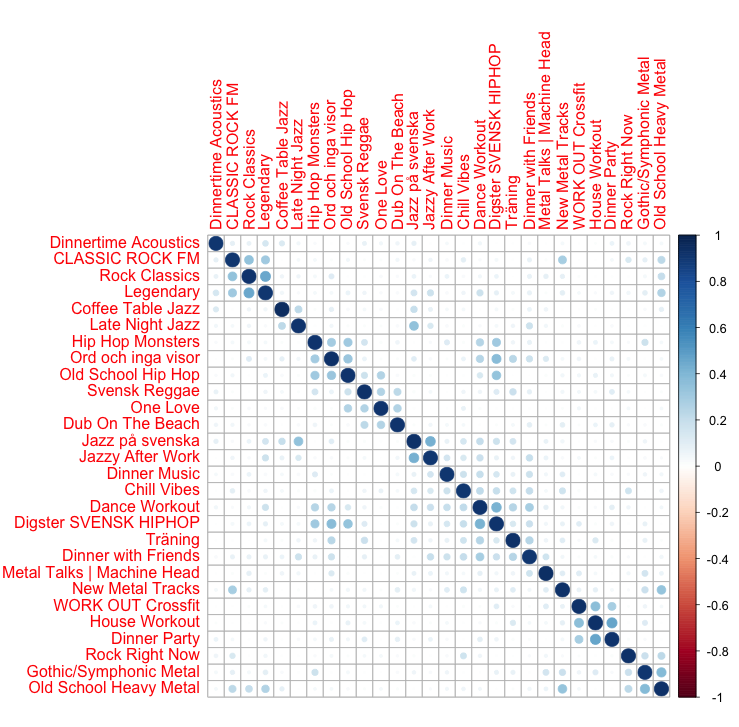
\includegraphics[scale=0.5]{images/absSum.png}
\caption{Hierarchical clustering of playlists where the aggregated measure of the weighted dot product matrix is taken by the absolute value of sum of the matrix diagonal. A look at the squares of correlation along the matrix diagonal shows interesting clusters. The three classical rock playlists in the data set are grouped together, three hip hop playlists are grouped into one cluster and so are three reggae playlists, there are two jazz clusters with two songs in each and there is also a workout/party cluster and a modern rock/metal cluster.}
\label{absSum}
\end{figure}

\begin{figure}
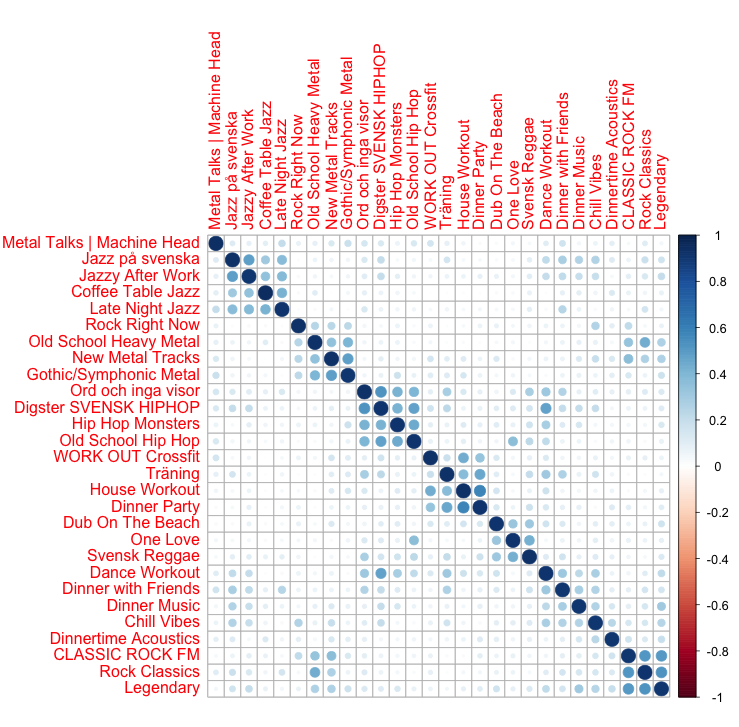
\includegraphics[scale=0.5]{images/sumAbs.png}
\caption{Hierarchical clustering of playlists where the aggregated measure of the weighted dot product matrix is taken by the sum of the absolute values of the matrix diagonal. The clusters along the diagonal using this method are more prominent than using the other methods. The clusters are easier to spot along the diagonal of the picture. The playlist comparison method used for this figure also does not provide several smaller clusters that are similar, such as two jazz clusters or two hip hop clusters as in \ref{sum} or \ref{absSum}}
\end{figure}


As can be seen summing the absolute values of the matrix diagonal provides a good clustering of similar playlists in the data set used. From a theoretical perspective summing the absolute values is also the method that makes the most sense. Eigenvectors from the covariance matrix explains the direction of variance, but it does not really matter if the variance is seen as going from A to B or from B to A. Hence the direction of eigenvectors from a playlist feature covariance matrix does not really matter. If the direction of eigenvectors do not matter then the resulting values of the matrix diagonal, provided by multiplying the weighted eigenvectors from two different playlist covariance matrices, do not matter either and it makes sense to use the sum of absolute values as an aggregated measure is used.

\section{Approximate Nearest Neighbours}
The major theoretical weakness of using Principal Component Analysis for finding latent factors of playlists is that PCA does not take location into consideration. PCA is an approximation of covariance in the data. When calculating covariance, the mean for each dimension in the data is subtracted from each data point. This operation is the same thing as normalizing or centering the data. Therefore when performing PCA the location of data is lost. Two sets of data, having the same relative variance among themselves, but located at two different places will have the same principal components despite having different location.

\begin{figure}
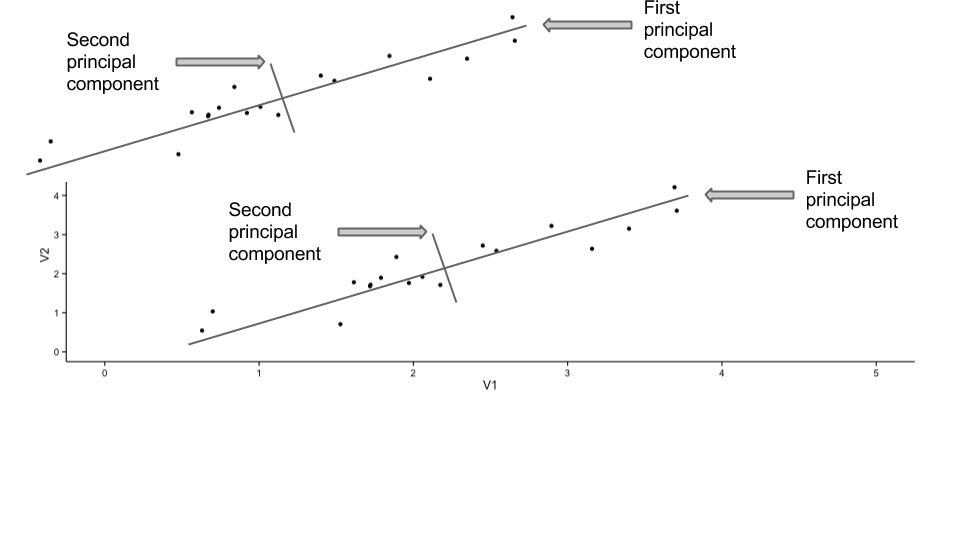
\includegraphics[scale=0.42]{images/pcaNormalize.png}
\caption{As can be seen the two data sets, if treated like independent data sets, have different location but still share the same principal components. This illustrates that information about location is thrown away by PCA. The information that is preserved is the direction, as the principal components show in which directions the variance in the data reside.}
\end{figure}



 An example of the theoretical weakness could be as follows: if the vector space used for describing tracks only consist of the genres Rock and Pop then a Rock playlist that varies from values ninety too one hundred in Rock and zero to ten in Pop and a Pop playlist with that varies from ninety to one hundred in Pop and zero to ten in Rock would have the same principal components. It can be argued that in the real case if two distinct playlists have the same principal components then they are either actually similar or badly described by their features. However the lack of capability of taking location into consideration is still a theoretical shortcoming that is intrinsic of the model. One remedy for this problem would be to add a pre-filtering step that would filter out tracks that are not located near the tracks of the seed playlist. The naive solution to this would be to use the nearest neighbours algorithm. The naive version of the nearest neighbour algorithm has two shortcomings. The first is that it has a quadratic complexity in the number of points, or tracks in this case, as each track is compared to every other track. The second shortcoming is that the algorithm needs a metric to calculate distance between points, such as the cosine similarity, and the calculation of distance for points becomes more expensive as the dimensionality of the vector space increases. For example if used with the cosine similarity nearest neighbours also has a quadratic complexity in the number of features. A solution with a quadratic complexity in the number of tracks quickly renders itself unfeasible if tracks are in the magnitude of millions and the operation needs to be done for every track in a seed playlist. 
Based on the notion that calculating distances in high dimensional vector spaces is an expensive procedure a solution is to compare points in lower dimensional spaces instead, by simply projecting the points into a space of lower dimensionality. The problem that arises here is that points that are distant in the original space might seem close in the subspace onto where they get projected. To make such confusions less probable several random subspace projections can be used. This technique is also known as Locality Sensitive Hashing, LSH.

\begin{figure}
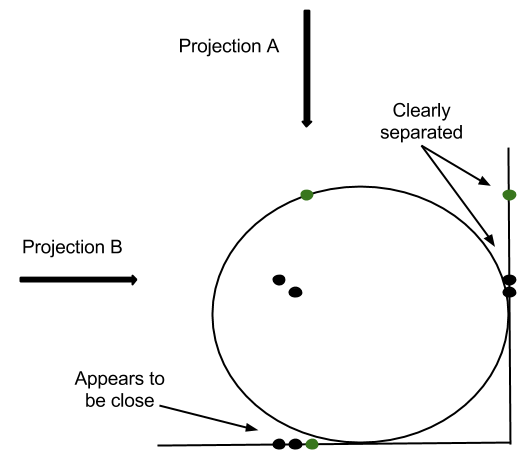
\includegraphics[scale=0.5]{images/LSH.png}
\caption{Illustration of random subspace projection. The illustration shows a concept that can be thought of as conceptually similar to both locality sensitive hashing and random separating hyperplanes}
\end{figure}

Locality Sensitive Hashing performs a good way of segmenting a high dimensional space into clusters. But scalability still remains an issue. One way of approximating the random subspace projections made by LSH is to deploy the use of random hyperplanes for separation. Random hyperplane segmentation for approximate nearest neighbours can be implemented by the use of several separating random hyperplanes. Each hyperplane is treated as a node in a binary tree as it separates all points into two categories. The segmentation made by one such tree is not necessarily optimal, but with several such trees an approximate nearest neighbour forest is obtained. Theoretically a higher number of trees in an approximate nearest neighbour forest should provide better segmentation of points up to a point on the magnitude of the number of relevant features in the data. Increasing the number of trees beyond this point would theoretically lead to a overly harsh discrimination and thus a less optimal segementation of data points. The time to retrieve the nearest neighbours of one point from approximate nearest neighbours is a constant time operation once the indexing of points is done. Thus by adding a approximate nearest neighbour pre-filtering step to the subspace method implies that subspace projections given an initial seed playlist only needs to be done for a subset of points from the whole data set.

This chapter has shown how principal component analysis, PCA, can be used to extract playlist characteristics. Subspace projections has been shown tp be applicable when selecting candidate tracks in the setting of playlist generation based on the components found by PCA. The information that is lost while doing PCA, the location, has been discussed and a method to take location into account, approximate nearest neighbours, has been presented. With this is mind the natural next step is to evaluate how this music recommendation pipeline performs which will be presented in the next chapter.

\chapter{Results}
\section{Precision}
Evaluating a generated playlist is a difficult task as there is no known ground truth for what a good playlist is. Even when asking normal persons or domain experts opinions about what consists a good playlist are likely to differ. There are of course sanctioned methods for evaluating data when features are present, using the cosine distance as an evaluation metric is one such approach. However using such as metric presents new problems. If the cosine distance, for example, is used for evaluation this would imply that the cosine distance also should also be used for the model. But if the evaluation metric and the objective function one tries to minimize are the same is there really an actual evaluation framework present or is the entire evaluation pipeline simply a tautology? Imagining the opposite is not compelling either. If one objective function is minimized by the model and another is used for evaluation one finds oneself in a situation of comparing apples and oranges, which is unlikely to be desired. Finding a way to evaluate generated playlists is without doubt a difficult task, but some metric is still needed as a proxy.
The first evaluation approach choosen for evaluating generated playlists finds its roots in the method of describing playlist similarity described in the methods section. 

\begin{figure}
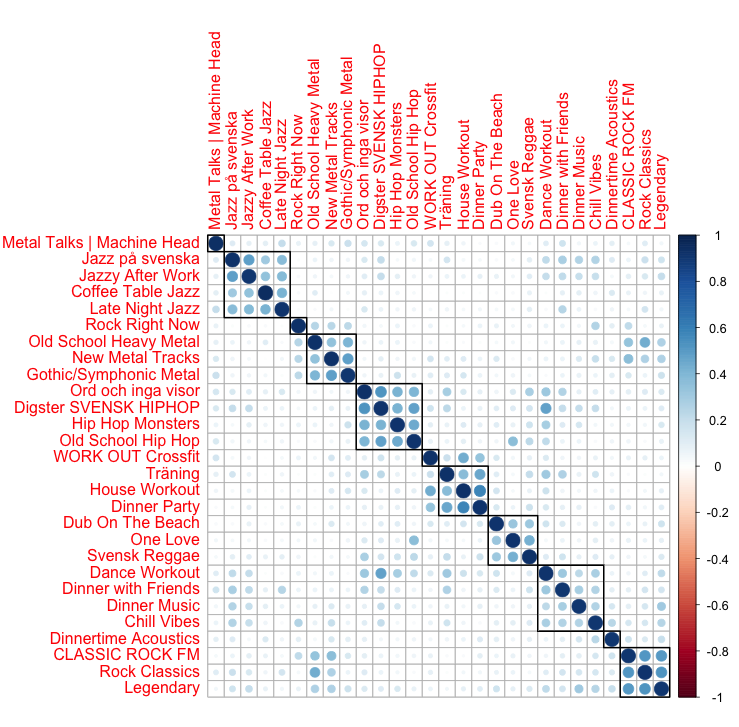
\includegraphics[scale=0.5]{images/sumAbsAgglHierClust-better.png}
\caption{Image showing the clustering used as a base for calculating precision. Clusters consisting of one single playlist were not used for evaluation.}
\label{sumAbsBetter}
\end{figure}


Based on the method of comparing playlists by taking the dot product of the principal components of two playlists, weighting by eigenvalues and transforming the resulting matrix into a scalar by summing the absolute values of the trace of the matrix an additional hierarchical clustering step can be added to create meaningful playlists clusters, as seen in \ref{sumAbsBetter}. As these clusters make up a sensible segmentation of playlists they where used as a base for evaluation. When the subspace method was applied to rank candidate songs for a seed playlist all songs that originates from a playlist within the same cluster as the seed playlist were considered true positives. All other songs were considered false positives. For the evaluation task a subset of data was used were only the tracks of the seven clusters consisting of more than one playlist from the figure above were used and pre-filtering was made by using approximate nearest neighbours with an euclidean distance measure. The approximate twenty nearest neighbours were used and the number of trees in each approximate nearest neighbour forest was varied. This is a non-optimal way of using approximate nearest neighbours as the proper way would be to select a by magnitude larger number of neighbours than actually needed, due to the fact that the method is an approximate. The reason for not doing doing so is that as small data set was used for evaluation using the two-hundred nearest neighbours would mean that the pre-filtering step would loose its effect as almost the entire data set would pass through pre-filtering. 
Precision was calculated for the ten, twenty and thirty top ranked songs. Calculating precision this way is a conservative measure as songs from playlists outside the cluster also might be good candidates. 

To give a reference to how the model performs a baseline is needed. What the model does is that it only takes part of the variance in playlist data into account. A reasonable baseline would therefor be to use a method that takes the full variance of data into account. A baseline that do this would be to use a random sample of songs after the initial approximate nearest neighbour step. This baseline was choosen and precision was calculated the same way as for the model. The evaluation then consists of one model only taking relevant variance into account and the other one considering the full variance of data. To account for randomness the random sampling was done ten times and the presented results are the averages of these ten sample sets.

\section{Comparing Model to Baseline}

\begin{figure}
\includegraphics[scale=0.08]{/Users/eaalto/Desktop/Latex/Master_Thesis_Report/images/boxplots/ggplot/no_jitter/model/p10_0outlierRmvd.png}
\includegraphics[scale=0.08]{/Users/eaalto/Desktop/Latex/Master_Thesis_Report/images/boxplots/ggplot/no_jitter/random/p10_0outlierRmvd.png}

\caption{Images showing how the model, left image, performs compared to the baseline, right image, for precision at 10.}
\end{figure}


\begin{figure}
\includegraphics[scale=0.08]{/Users/eaalto/Desktop/Latex/Master_Thesis_Report/images/boxplots/ggplot/no_jitter/model/p20_0outlierRmvd.png}
\includegraphics[scale=0.08]{/Users/eaalto/Desktop/Latex/Master_Thesis_Report/images/boxplots/ggplot/no_jitter/random/p20_0outlierRmvd.png}
\caption{Images showing how the model, left image, performs compared to the baseline, right image, for precision at 20.}
\end{figure}

\begin{figure}
\includegraphics[scale=0.08]{/Users/eaalto/Desktop/Latex/Master_Thesis_Report/images/boxplots/ggplot/no_jitter/model/p30_0outlierRmvd.png}
\includegraphics[scale=0.08]{/Users/eaalto/Desktop/Latex/Master_Thesis_Report/images/boxplots/ggplot/no_jitter/random/p30_0outlierRmvd.png}
\caption{Images showing how the model, left image, performs compared to the baseline, right image, for precision at 30.}
\end{figure}

As can be seen the model outperforms the baseline in some cases by an increase in precision hundred percent or more and never performs less than twenty five percent better than the baseline, on average. 
When increasing the number of trees in the approximate nearest neighbour pre-filtering step while using the model the lower limit of variance goes down. This implies that using approximate nearest neighbours as pre-filtering discriminates tracks that are true positives. To scrutinize this lets look more closely at the data and see how the data points are distributed along the axis of variance.

\begin{figure}
\includegraphics[scale=0.1]{/Users/eaalto/Desktop/Latex/Master_Thesis_Report/images/boxplots/ggplot/p10_0outlierRmvd.png}

\caption{Image showing the averages including data points for precision at 10}
\end{figure}

\begin{figure}
\includegraphics[scale=0.1]{/Users/eaalto/Desktop/Latex/Master_Thesis_Report/images/boxplots/ggplot/p20_0outlierRmvd.png}
\caption{Image showing the averages including data points for precision at 20}
\end{figure}


\begin{figure}
Model@30
\includegraphics[scale=0.1]{/Users/eaalto/Desktop/Latex/Master_Thesis_Report/images/boxplots/ggplot/p30_0outlierRmvd.png}
\caption{Image showing the averages including data points for precision at 30}
\end{figure}

What can be seen is that there is only one point that causes the lower tail in variance for each boxplot, this point is a result of the same playlist for each boxplot and is also the overall lowest performing playlist. This point can therefore be threated as an outlier as it is not well described by the model. Removing this outlier yields the following result.

\begin{figure}
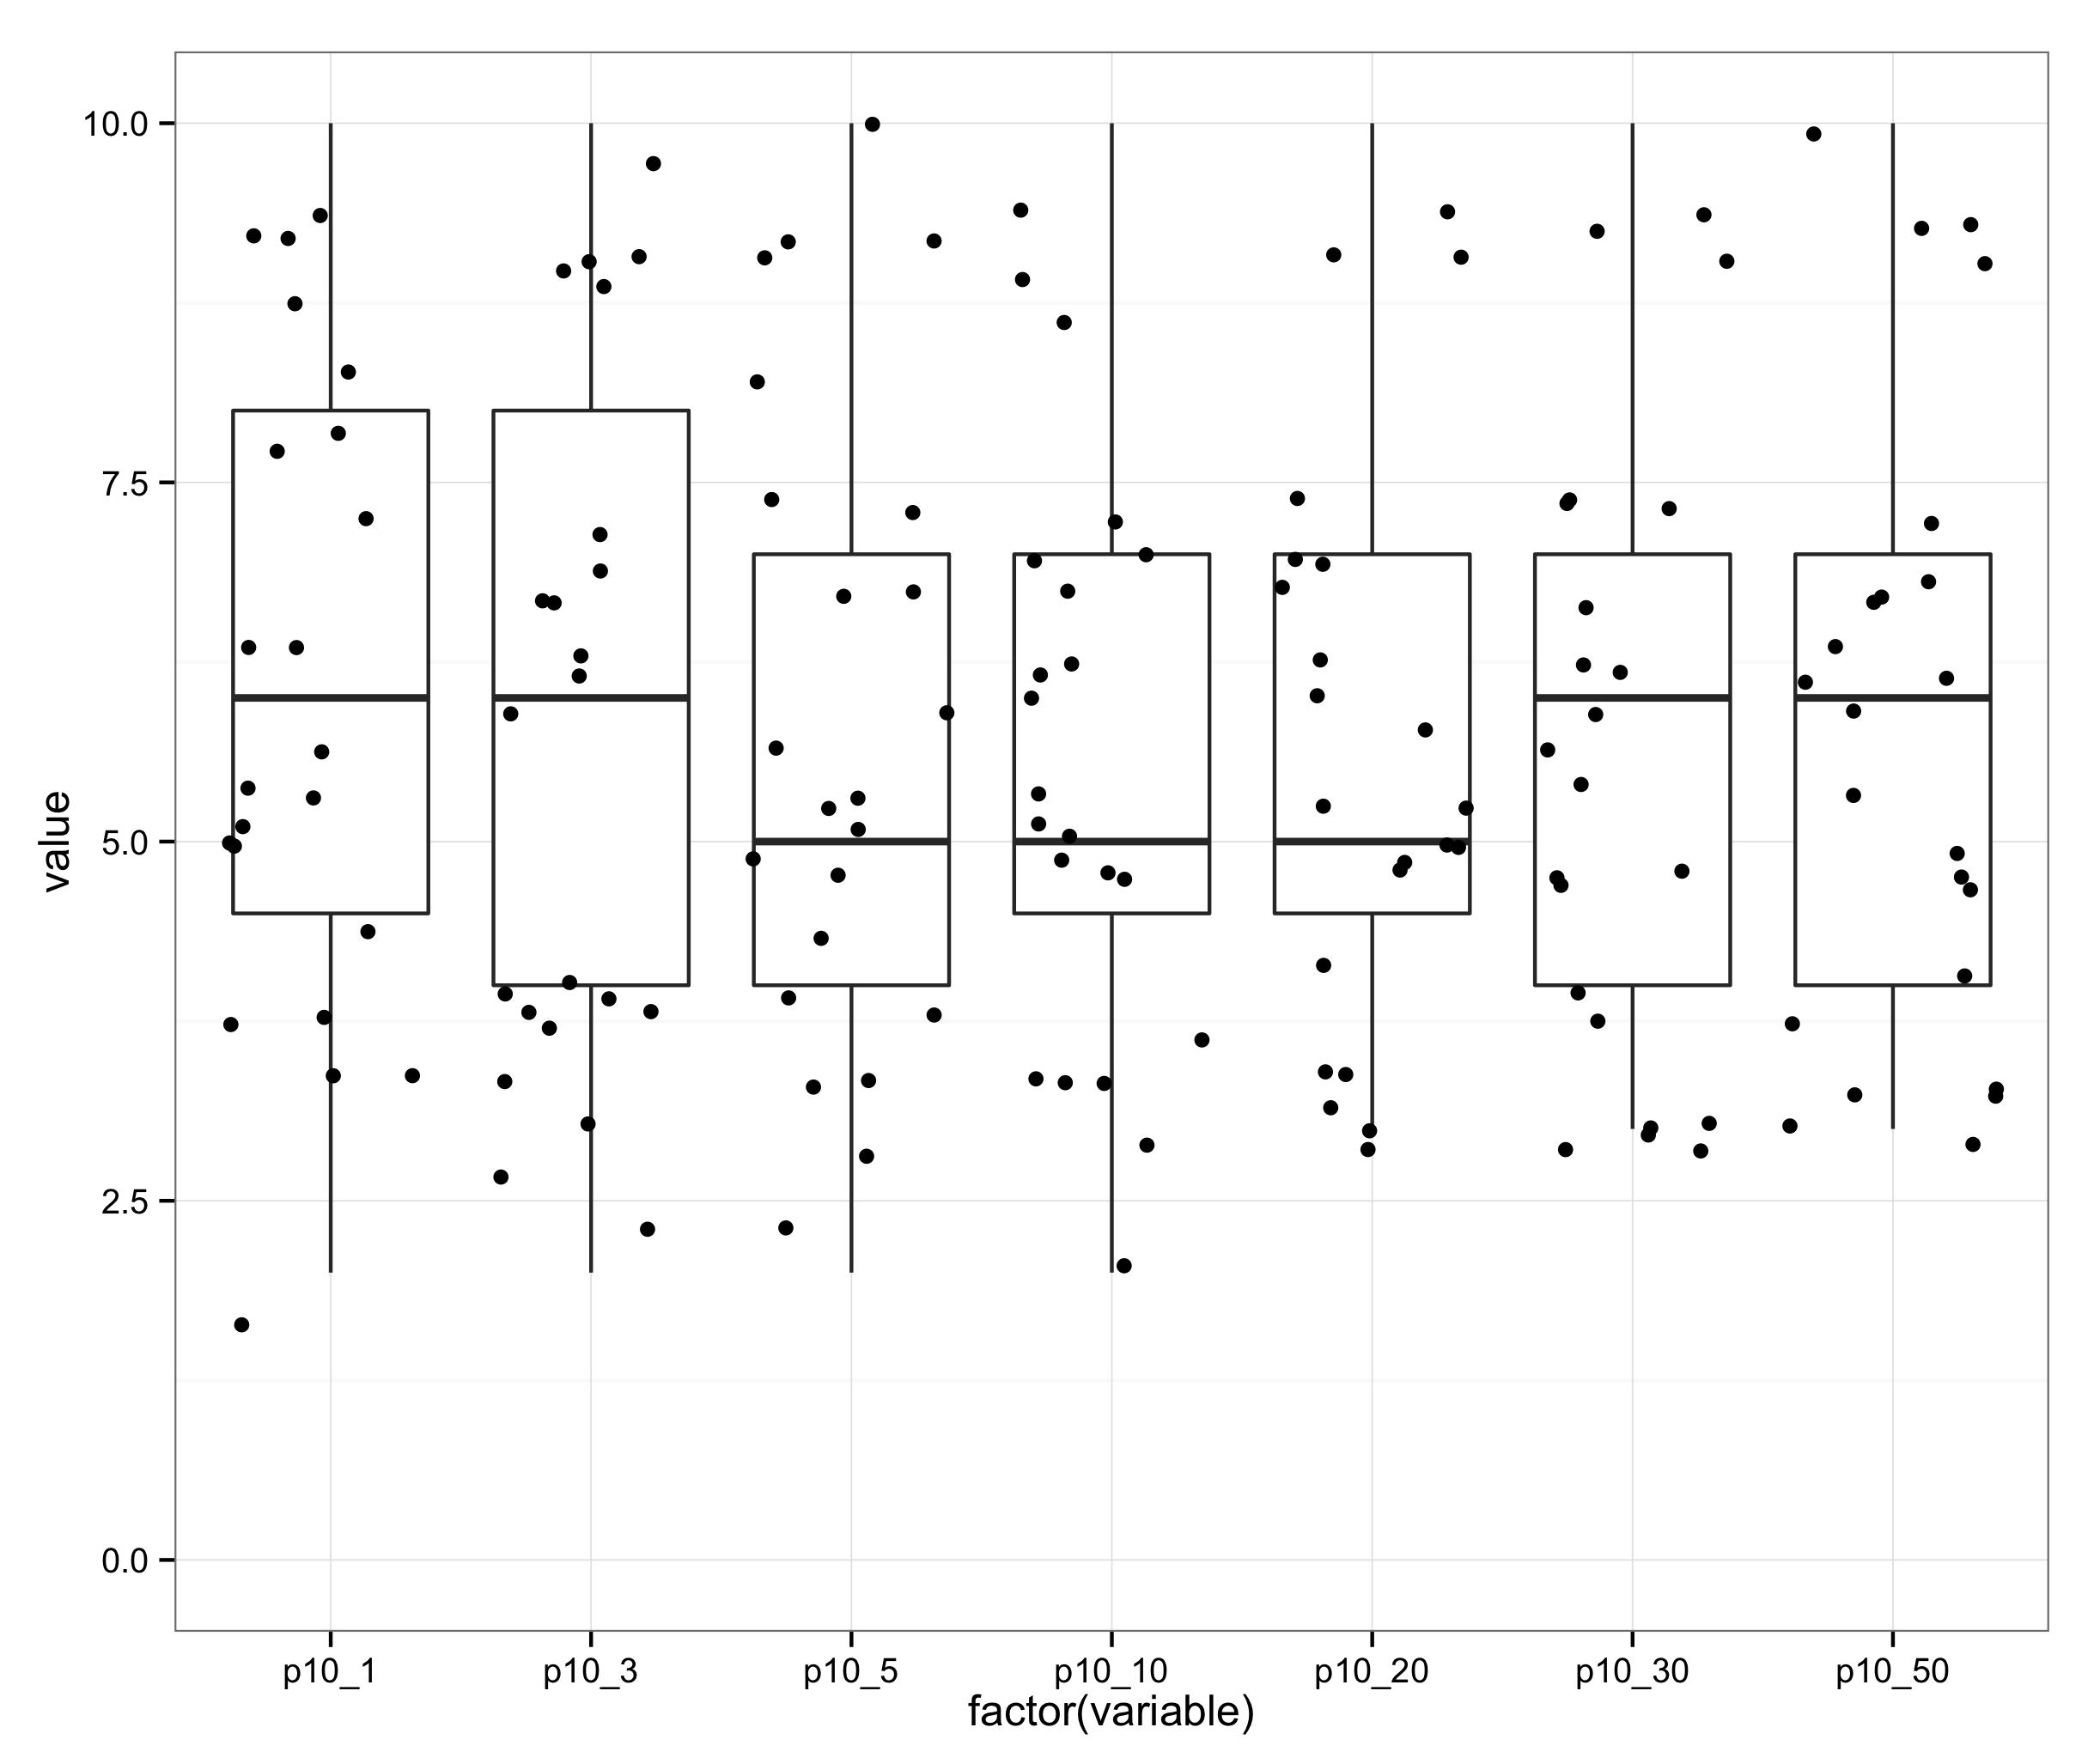
\includegraphics[scale=0.1]{/Users/eaalto/Desktop/Latex/Master_Thesis_Report/images/boxplots/ggplot/p10_1outlierRmvd.png}
\caption{Image showing the averages including data points for precision at 10 with one outlier removed}
\end{figure}

\begin{figure}
Model@20 1 outlier removed
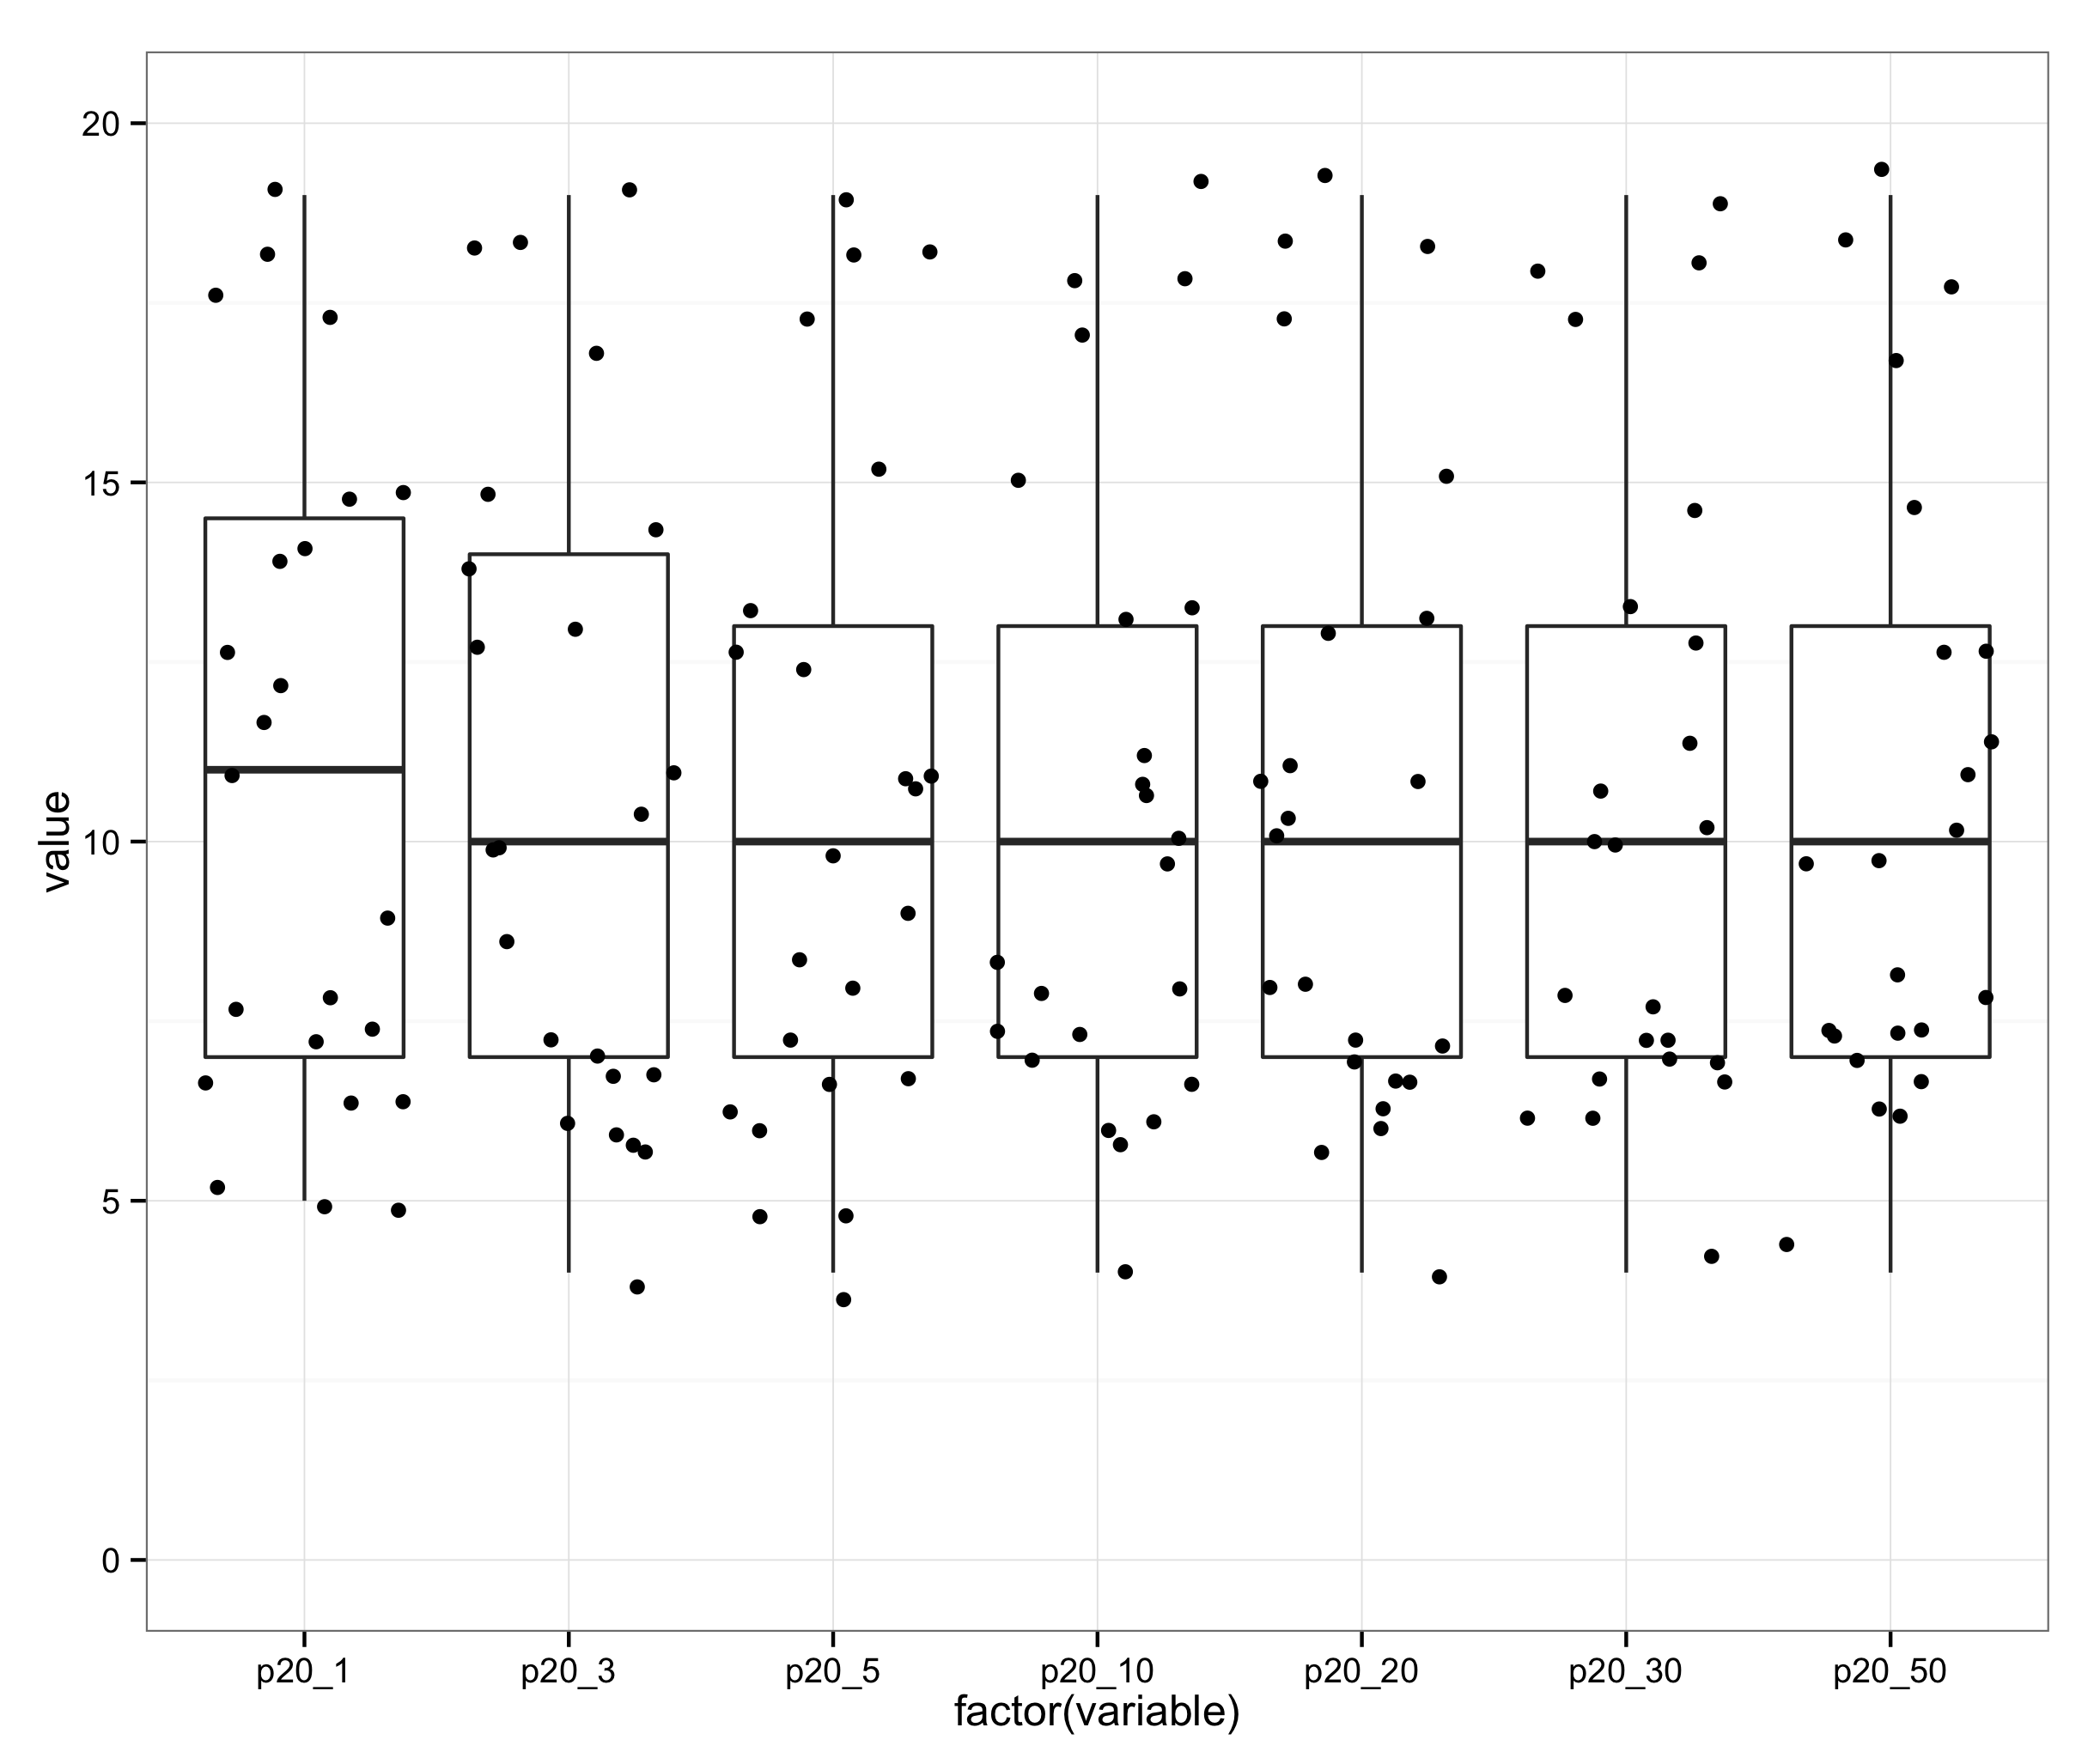
\includegraphics[scale=0.1]{/Users/eaalto/Desktop/Latex/Master_Thesis_Report/images/boxplots/ggplot/p20_1outlierRmvd.png}
\caption{Image showing the averages including data points for precision at 20 with one outlier removed}
\end{figure}

\begin{figure}
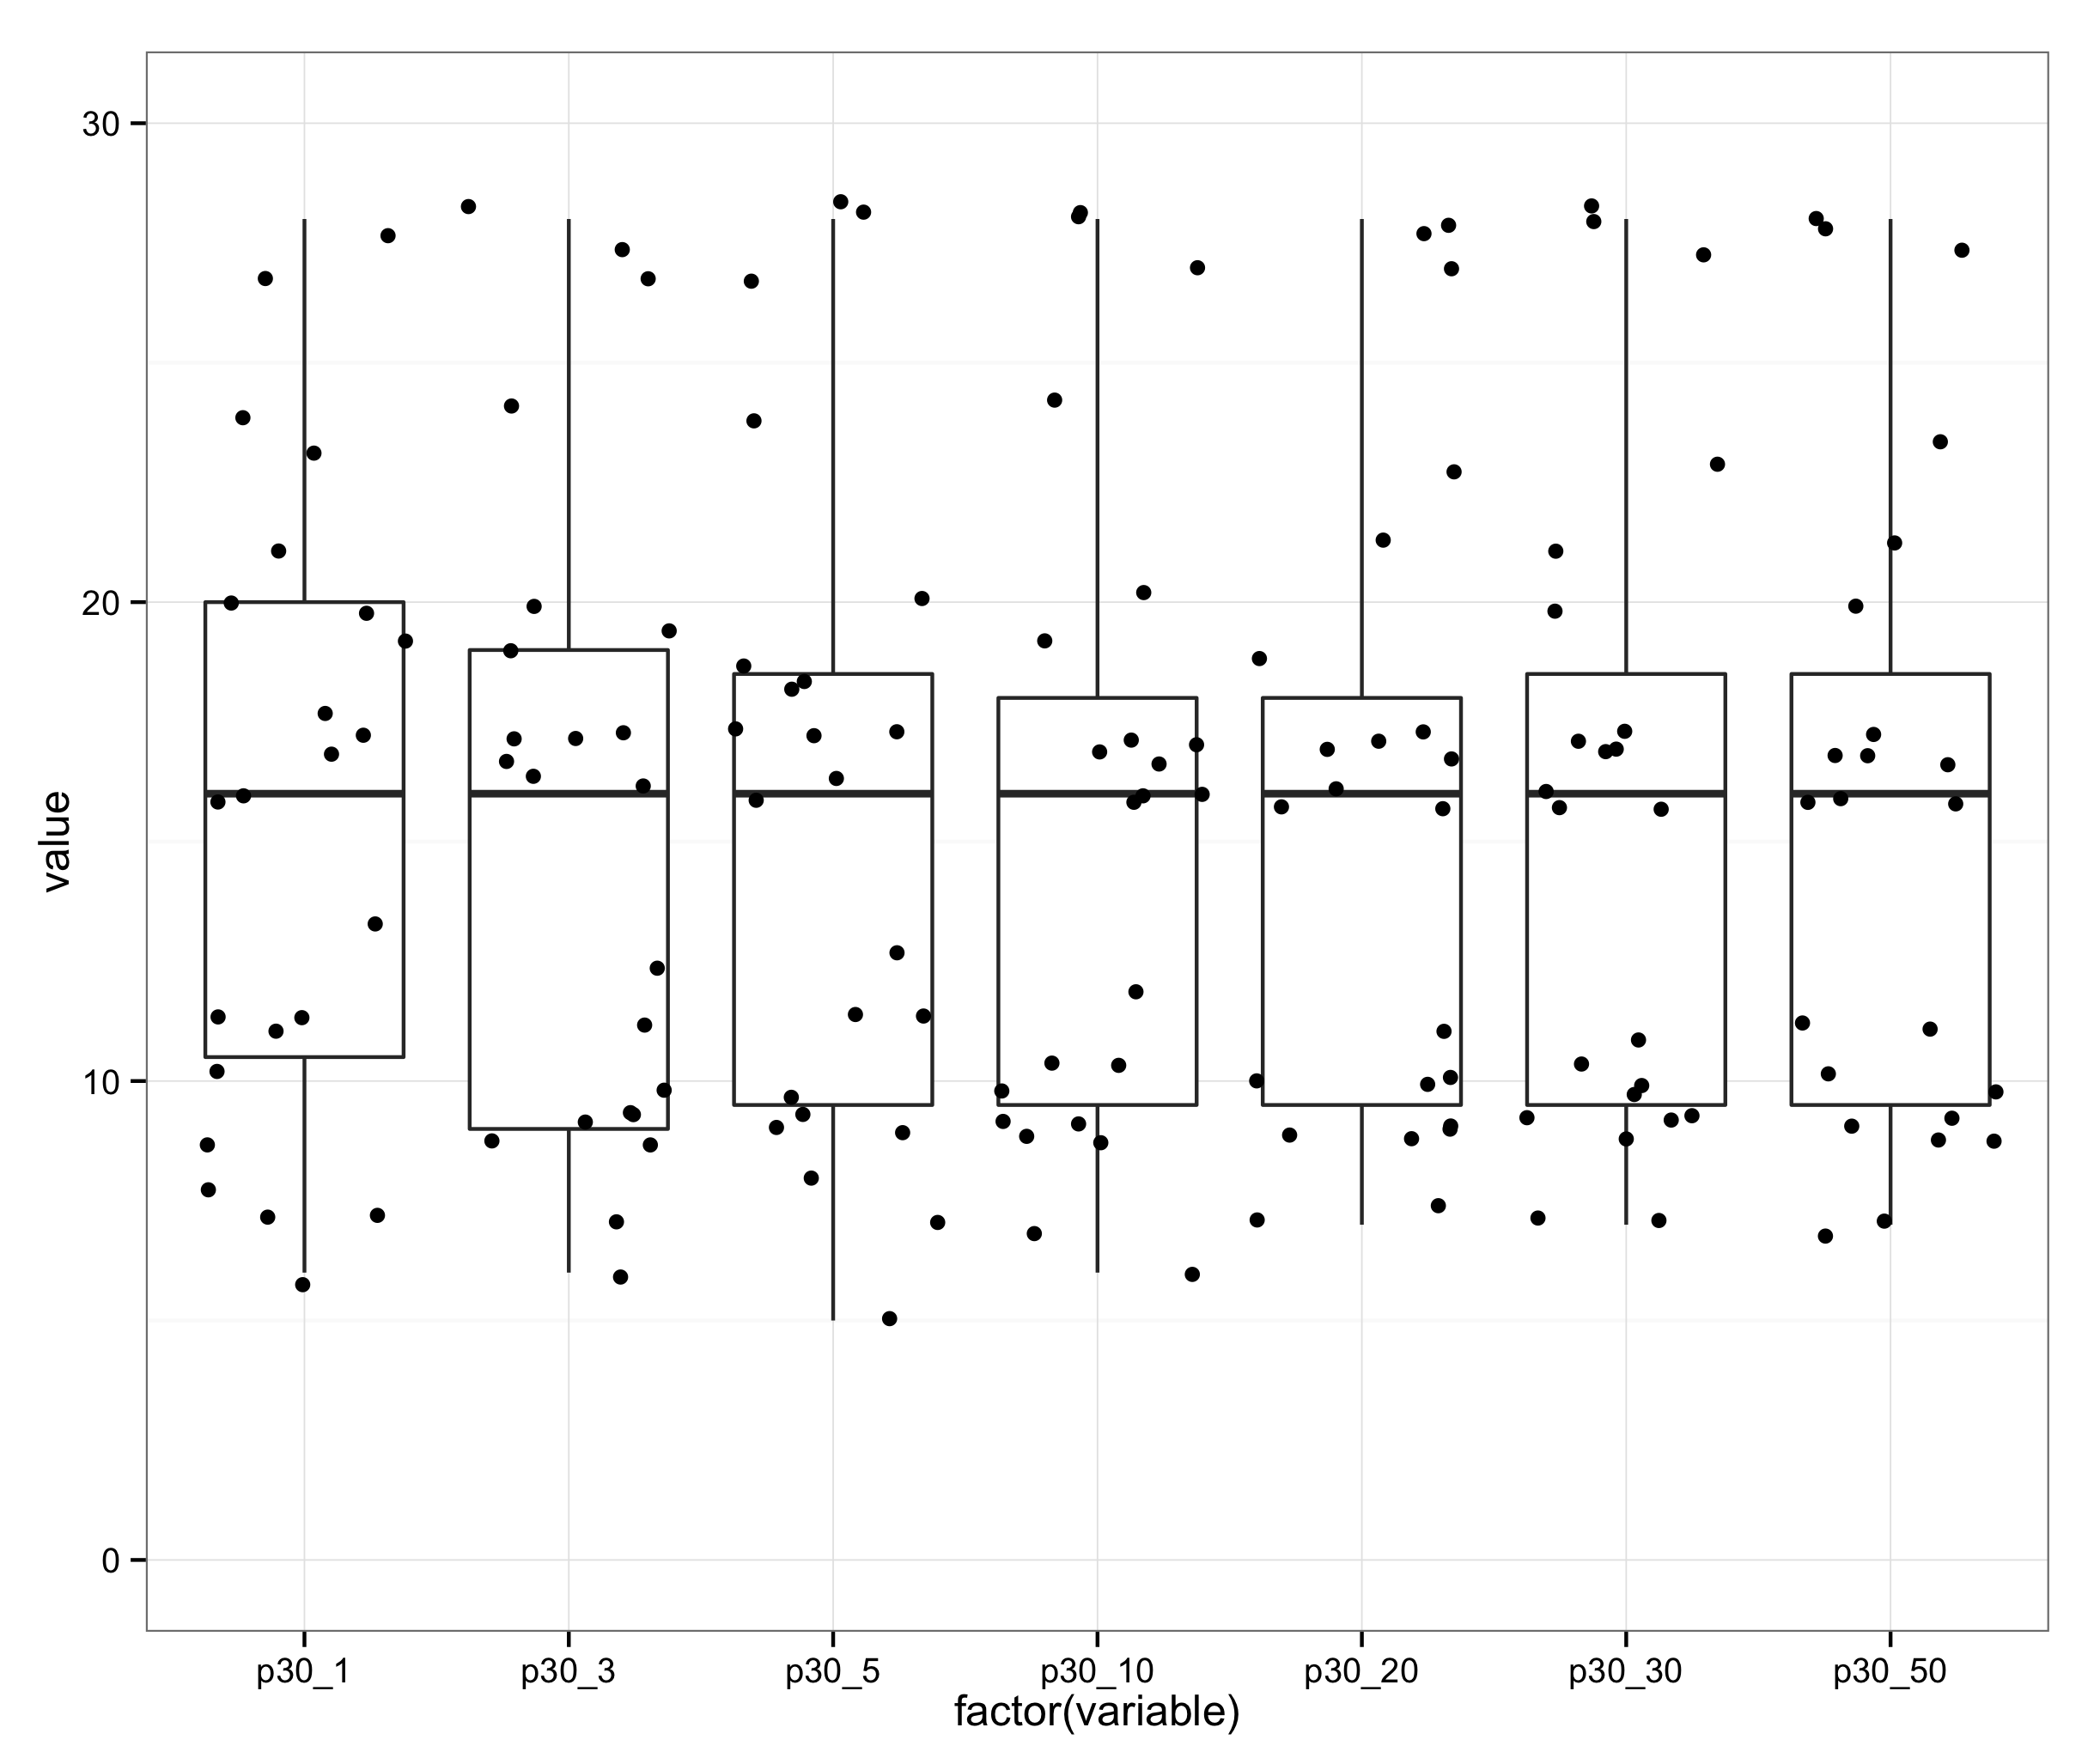
\includegraphics[scale=0.1]{/Users/eaalto/Desktop/Latex/Master_Thesis_Report/images/boxplots/ggplot/p30_1outlierRmvd.png}
\caption{Image showing the averages including data points for precision at 30 with one outlier removed}
\end{figure}


With the outlier removed the lower tail of variance is stable or decreasing as the number of trees in the pre-filtering step increase. As increasing the number of trees while pre-filtering leads to a higher discrimination the plausible decrease in variance is coherent with theory. There is also a fluctuation in precision as the number of trees varies, but without a clear trend. Removing one outlier also alters how the precision varies, what this entails is that the amount of data used for these experiments is not enough to draw conclusions regarding a trend in precision as a function of the number of trees used in pre-filtering. The fluctuations in precision are to be regarded as pecularities in the data set rather than ground for generalized conclusions as no clear trend can be spotted.

\section{Confusions}
As can be seen in the image showing the playlist clusters there is often a high correlation between a playlist inside a cluster and another playlist outside the cluster, as for example between the playlists \textit{Digster SVENSK HIPHOP} and \textit{Dance Workout}. Using precision by only considering tracks from playlists inside the clusters as true positives is therefore a conservative measure and the actual results might therefore be better than what the precision results entail. To quantify and investigate to what extent false postives come from closely related playlists histograms of the rank of playlists from which the false postive tracks originated were made. Here the rank is the rank of how highly ranked the playlist the false positive sample originated from was related to the seed playlist for the entire data set. That is, for each playlist in the data set a ranking of all playlists in terms of similarity in their principal component spaces, as performed when comparing playlists earlier, is made. Once this ranking is made for each playlist, all tracks classified as false positives when calculating the precision for a seed playlist are mapped to the rank of the playlist, from which the false positive originates, when compared to the seed playlist. Once this is done all these ranks are saved. To visualize the distribution of these ranks histograms were made for all number of trees for the approximate nearest neighbour pre-filtering step.

\begin{figure}
1 tree
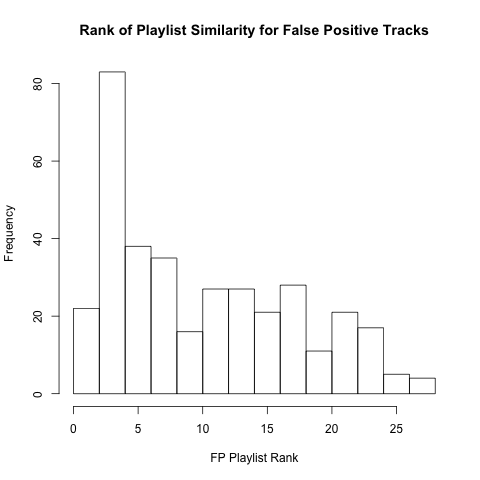
\includegraphics[scale=0.4]{/Users/eaalto/Desktop/Latex/Master_Thesis_Report/images/confRanks/confRankPlot1.png}
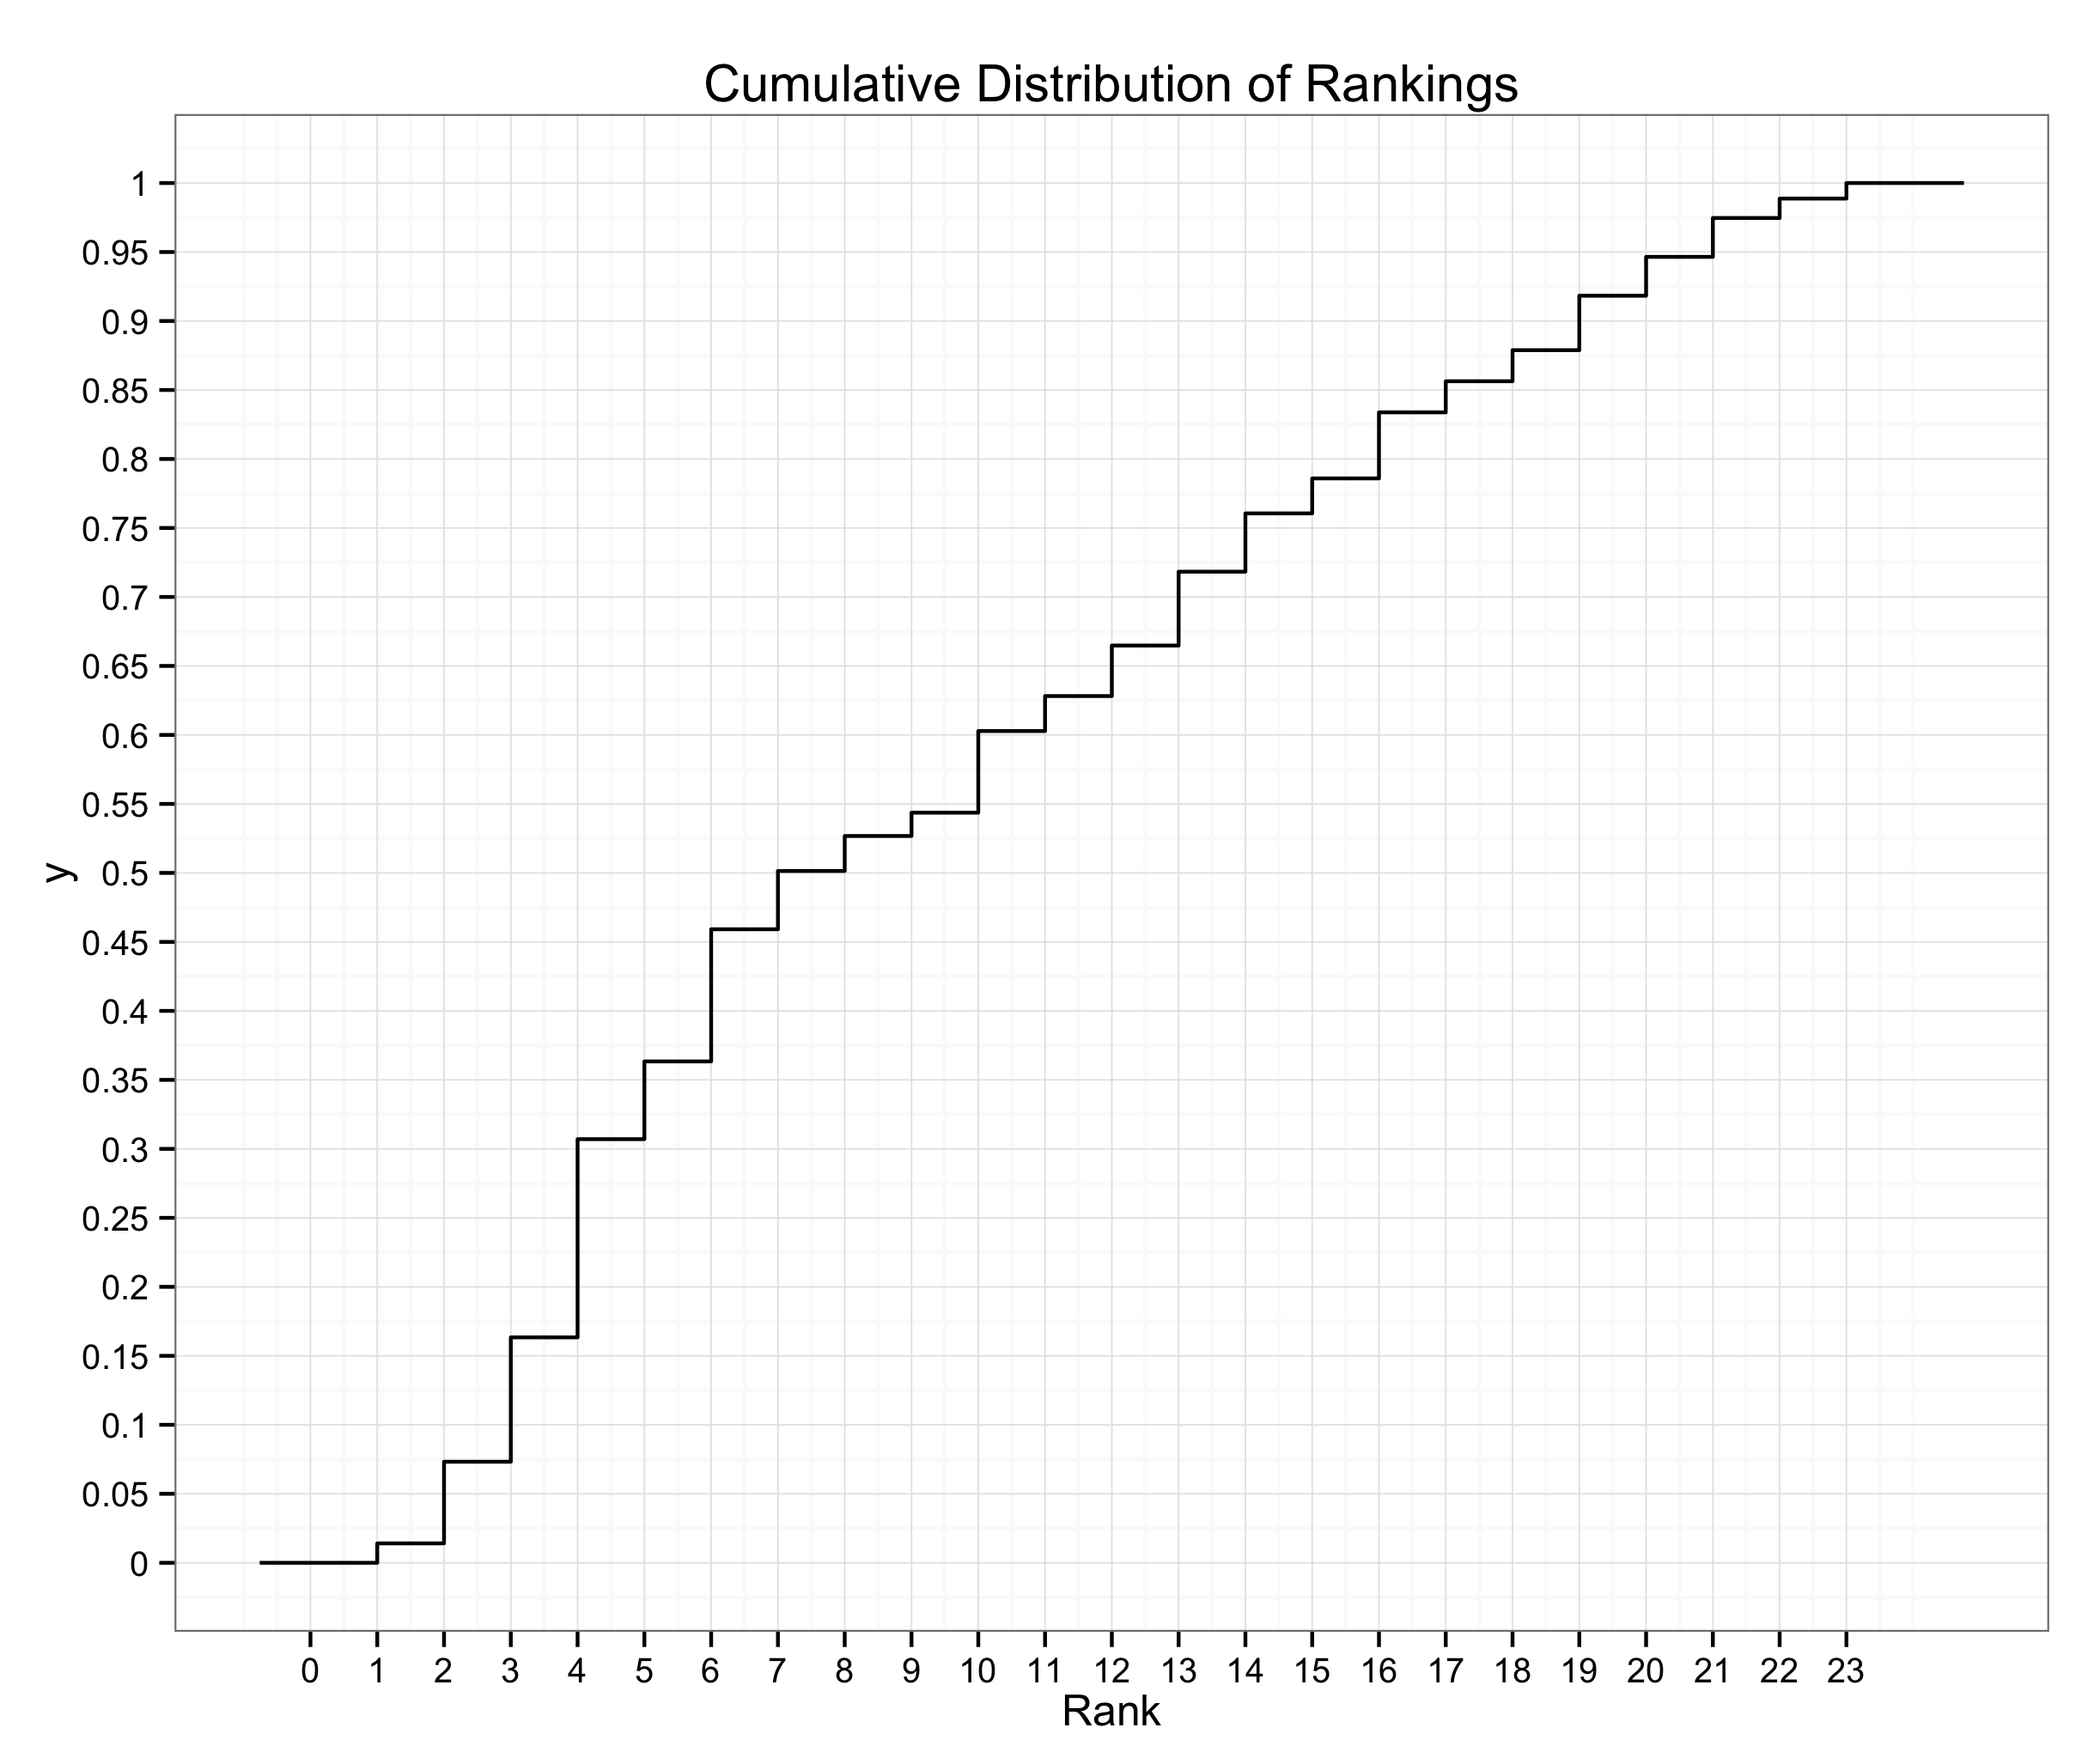
\includegraphics[scale=0.1]{/Users/eaalto/Desktop/Latex/Master_Thesis_Report/images/confRanks/confRankCumSum1.png}
\caption{Image to the left showing a histogram over similarity ranks to the seed playlists, for the playlists to which the false positive samples belong. The figure to the right shows the cumulative distribution of rankings. Both figures show performance for 1 tree in the pre-filtering step.}
\end{figure}

\begin{figure}
3 trees
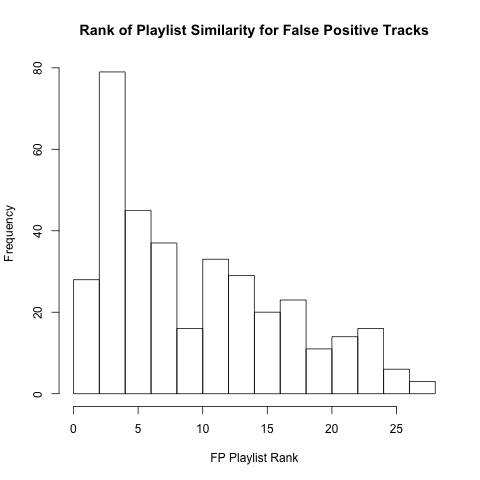
\includegraphics[scale=0.4]{/Users/eaalto/Desktop/Latex/Master_Thesis_Report/images/confRanks/confRankPlot3.png}
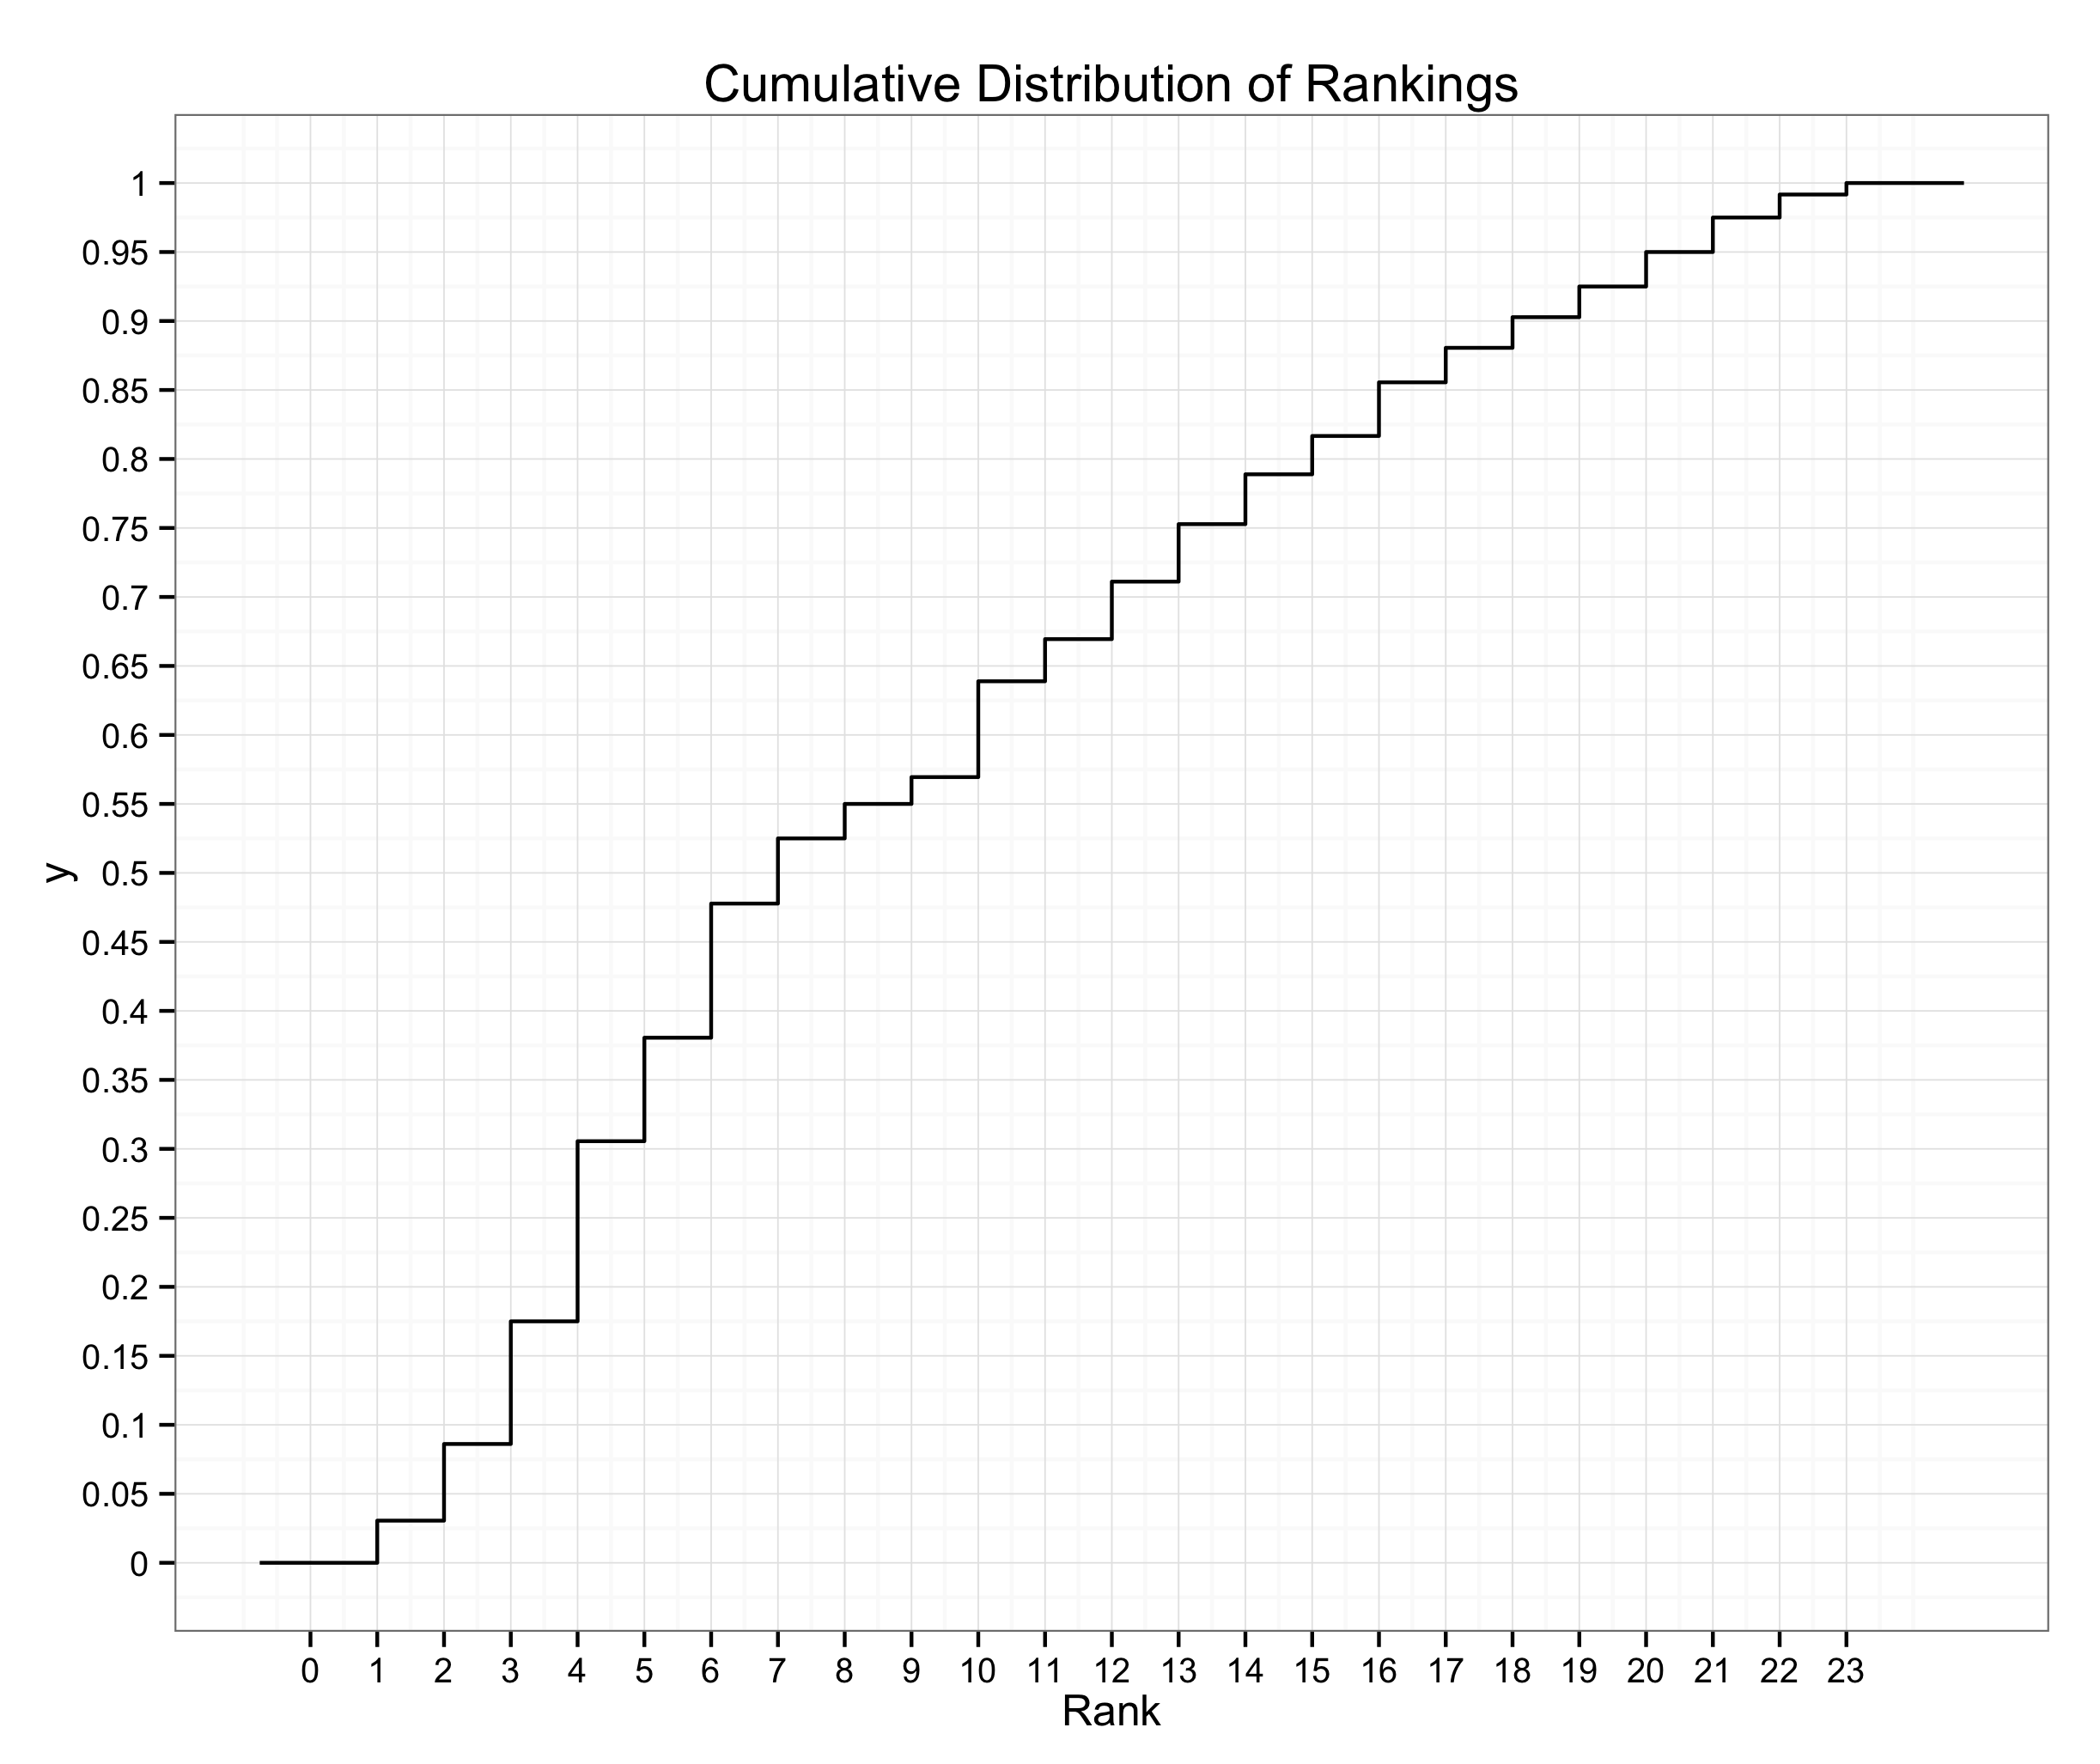
\includegraphics[scale=0.1]{/Users/eaalto/Desktop/Latex/Master_Thesis_Report/images/confRanks/confRankCumSum3.png}
\caption{Image to the left showing a histogram over similarity ranks to the seed playlists, for the playlists to which the false positive samples belong. The figure to the right shows the cumulative distribution of rankings. Both figures show performance for 3 trees in the pre-filtering step.}
\end{figure}

\begin{figure}
5 trees
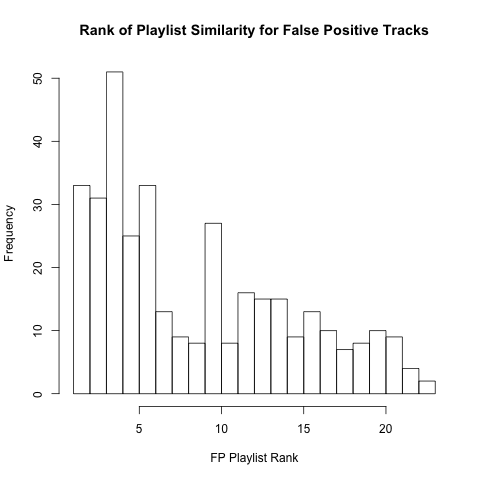
\includegraphics[scale=0.4]{/Users/eaalto/Desktop/Latex/Master_Thesis_Report/images/confRanks/confRankPlot5.png}
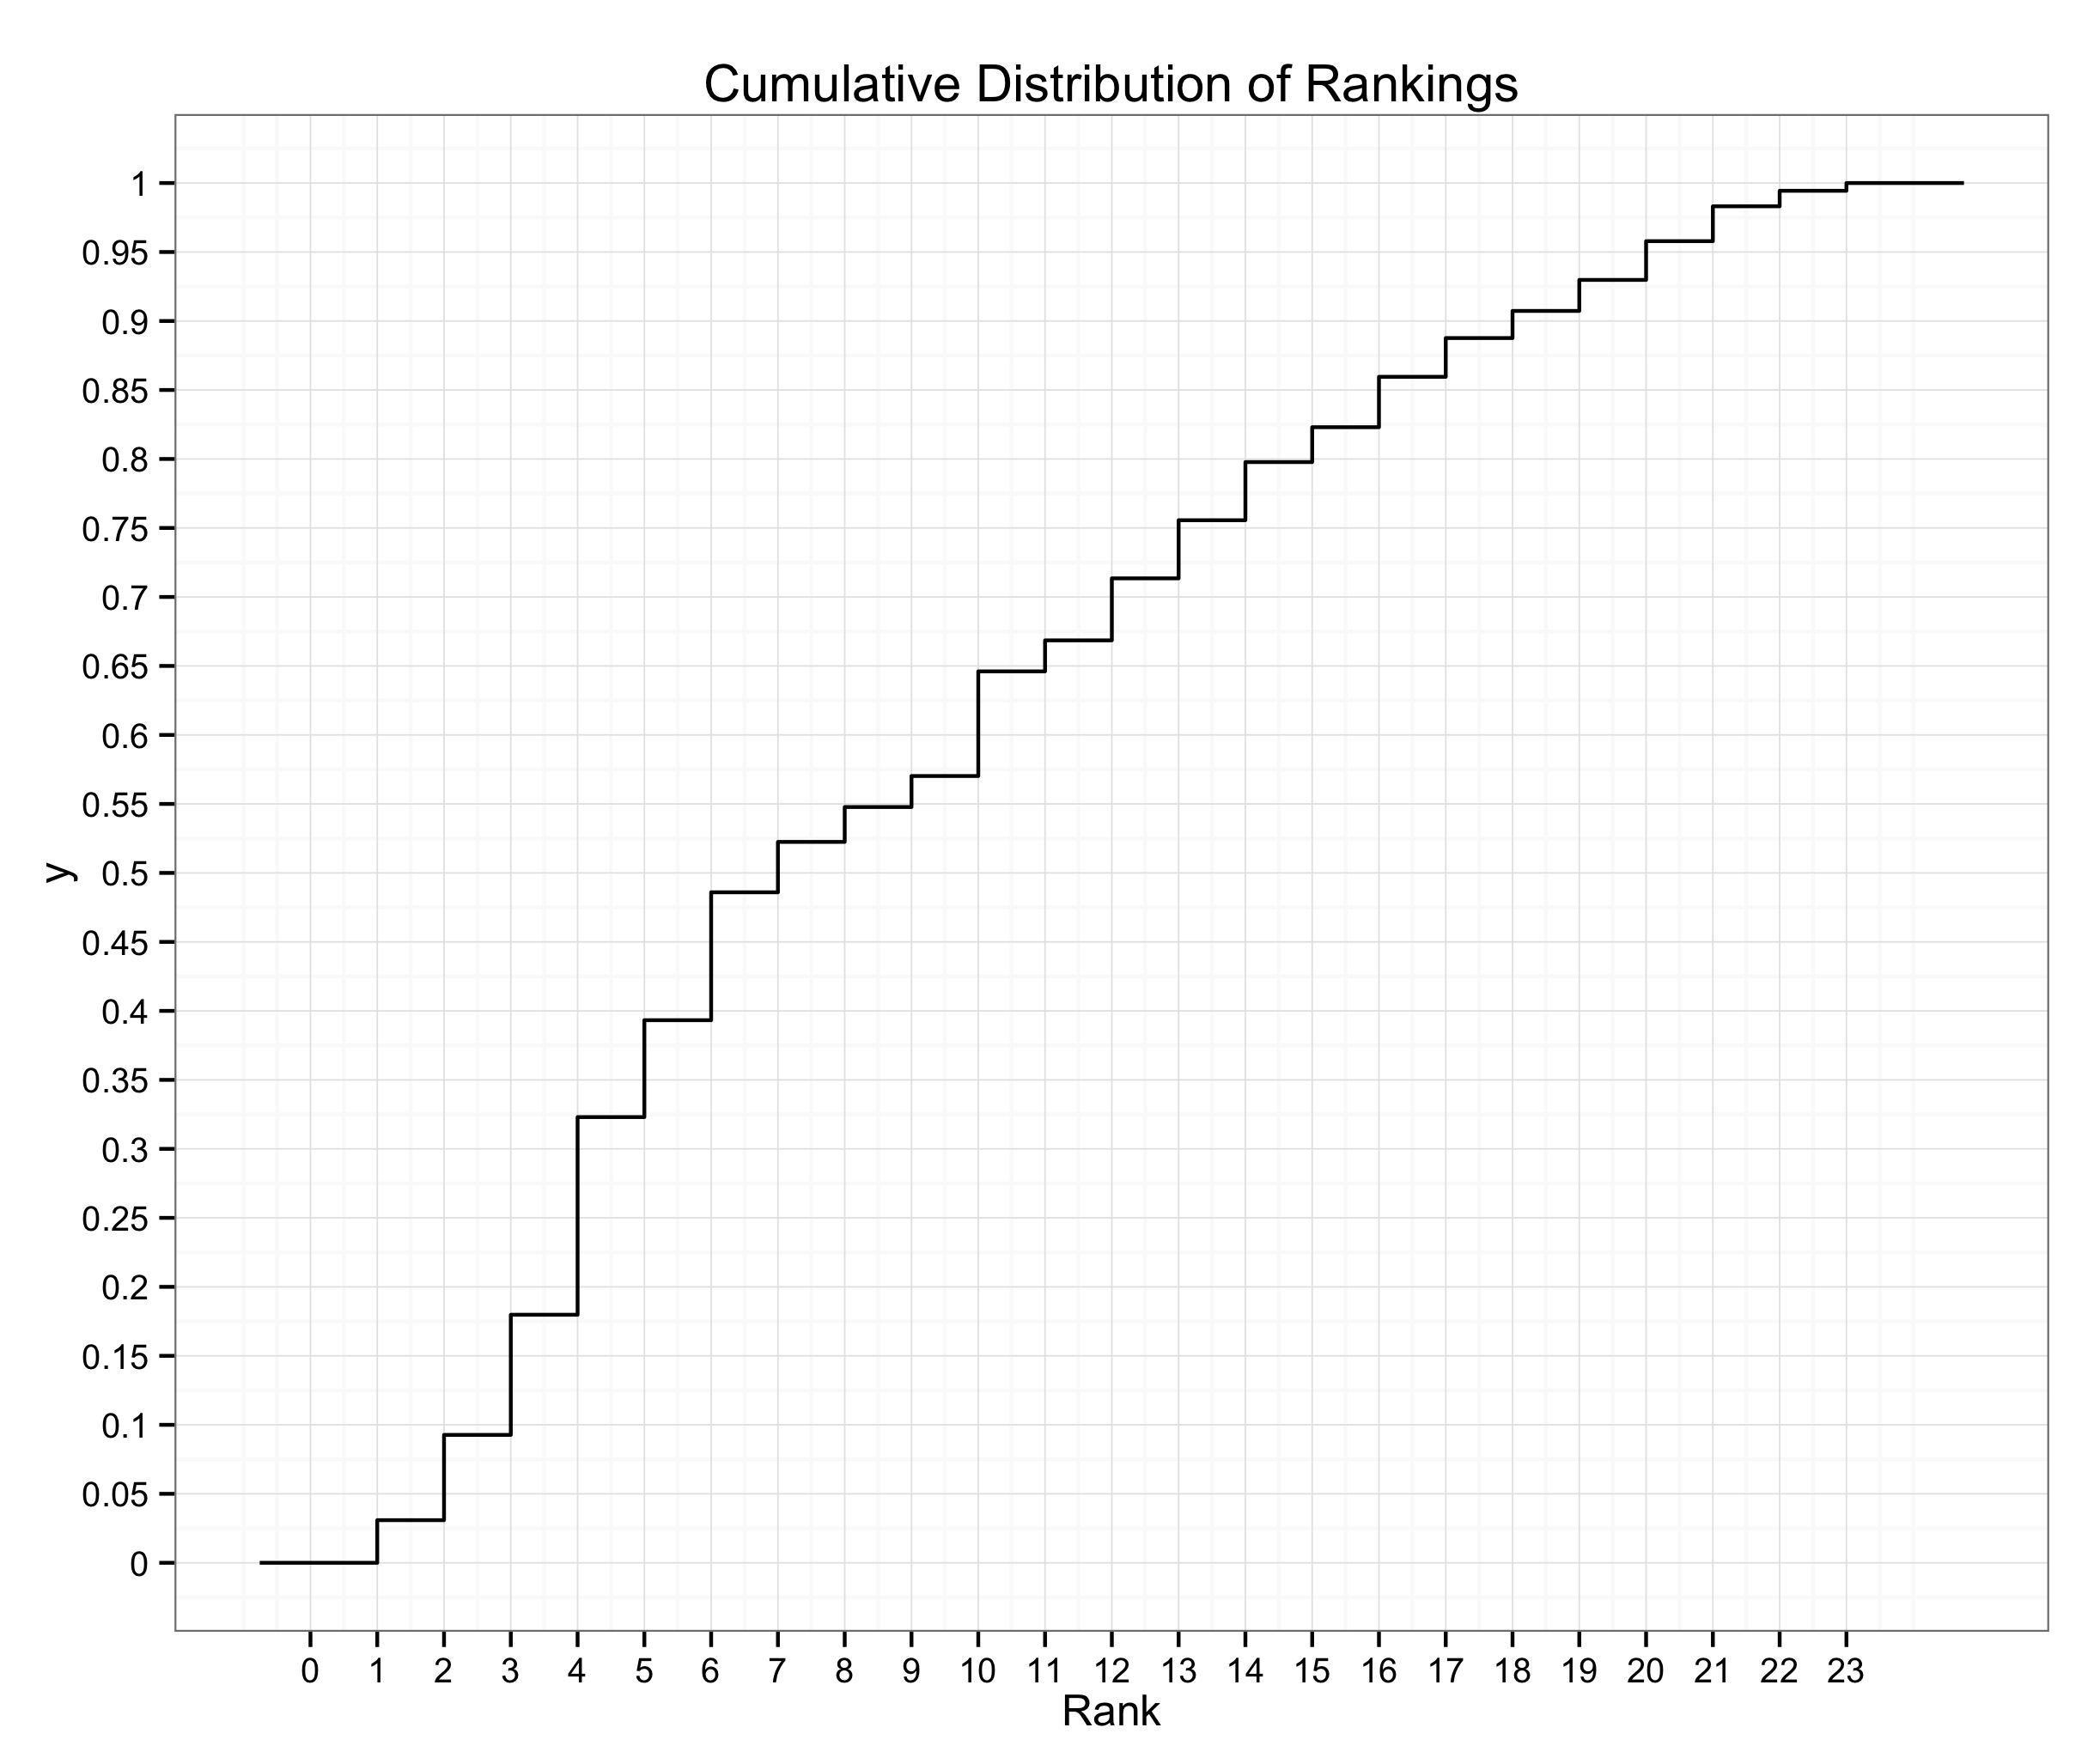
\includegraphics[scale=0.1]{/Users/eaalto/Desktop/Latex/Master_Thesis_Report/images/confRanks/confRankCumSum5.png}
\caption{Image to the left showing a histogram over similarity ranks to the seed playlists, for the playlists to which the false positive samples belong. The figure to the right shows the cumulative distribution of rankings. Both figures show performance for 5 trees in the pre-filtering step.}
\end{figure}

\begin{figure}
10 trees
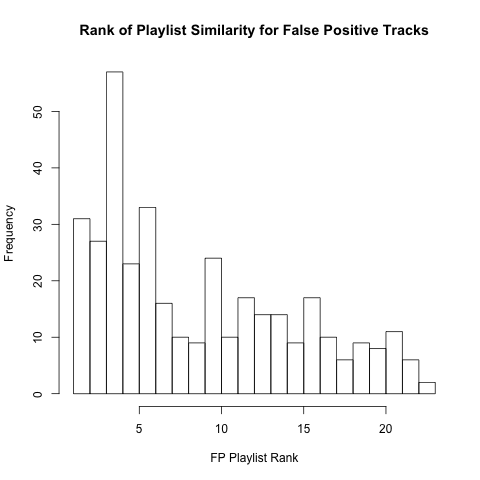
\includegraphics[scale=0.4]{/Users/eaalto/Desktop/Latex/Master_Thesis_Report/images/confRanks/confRankPlot10.png}
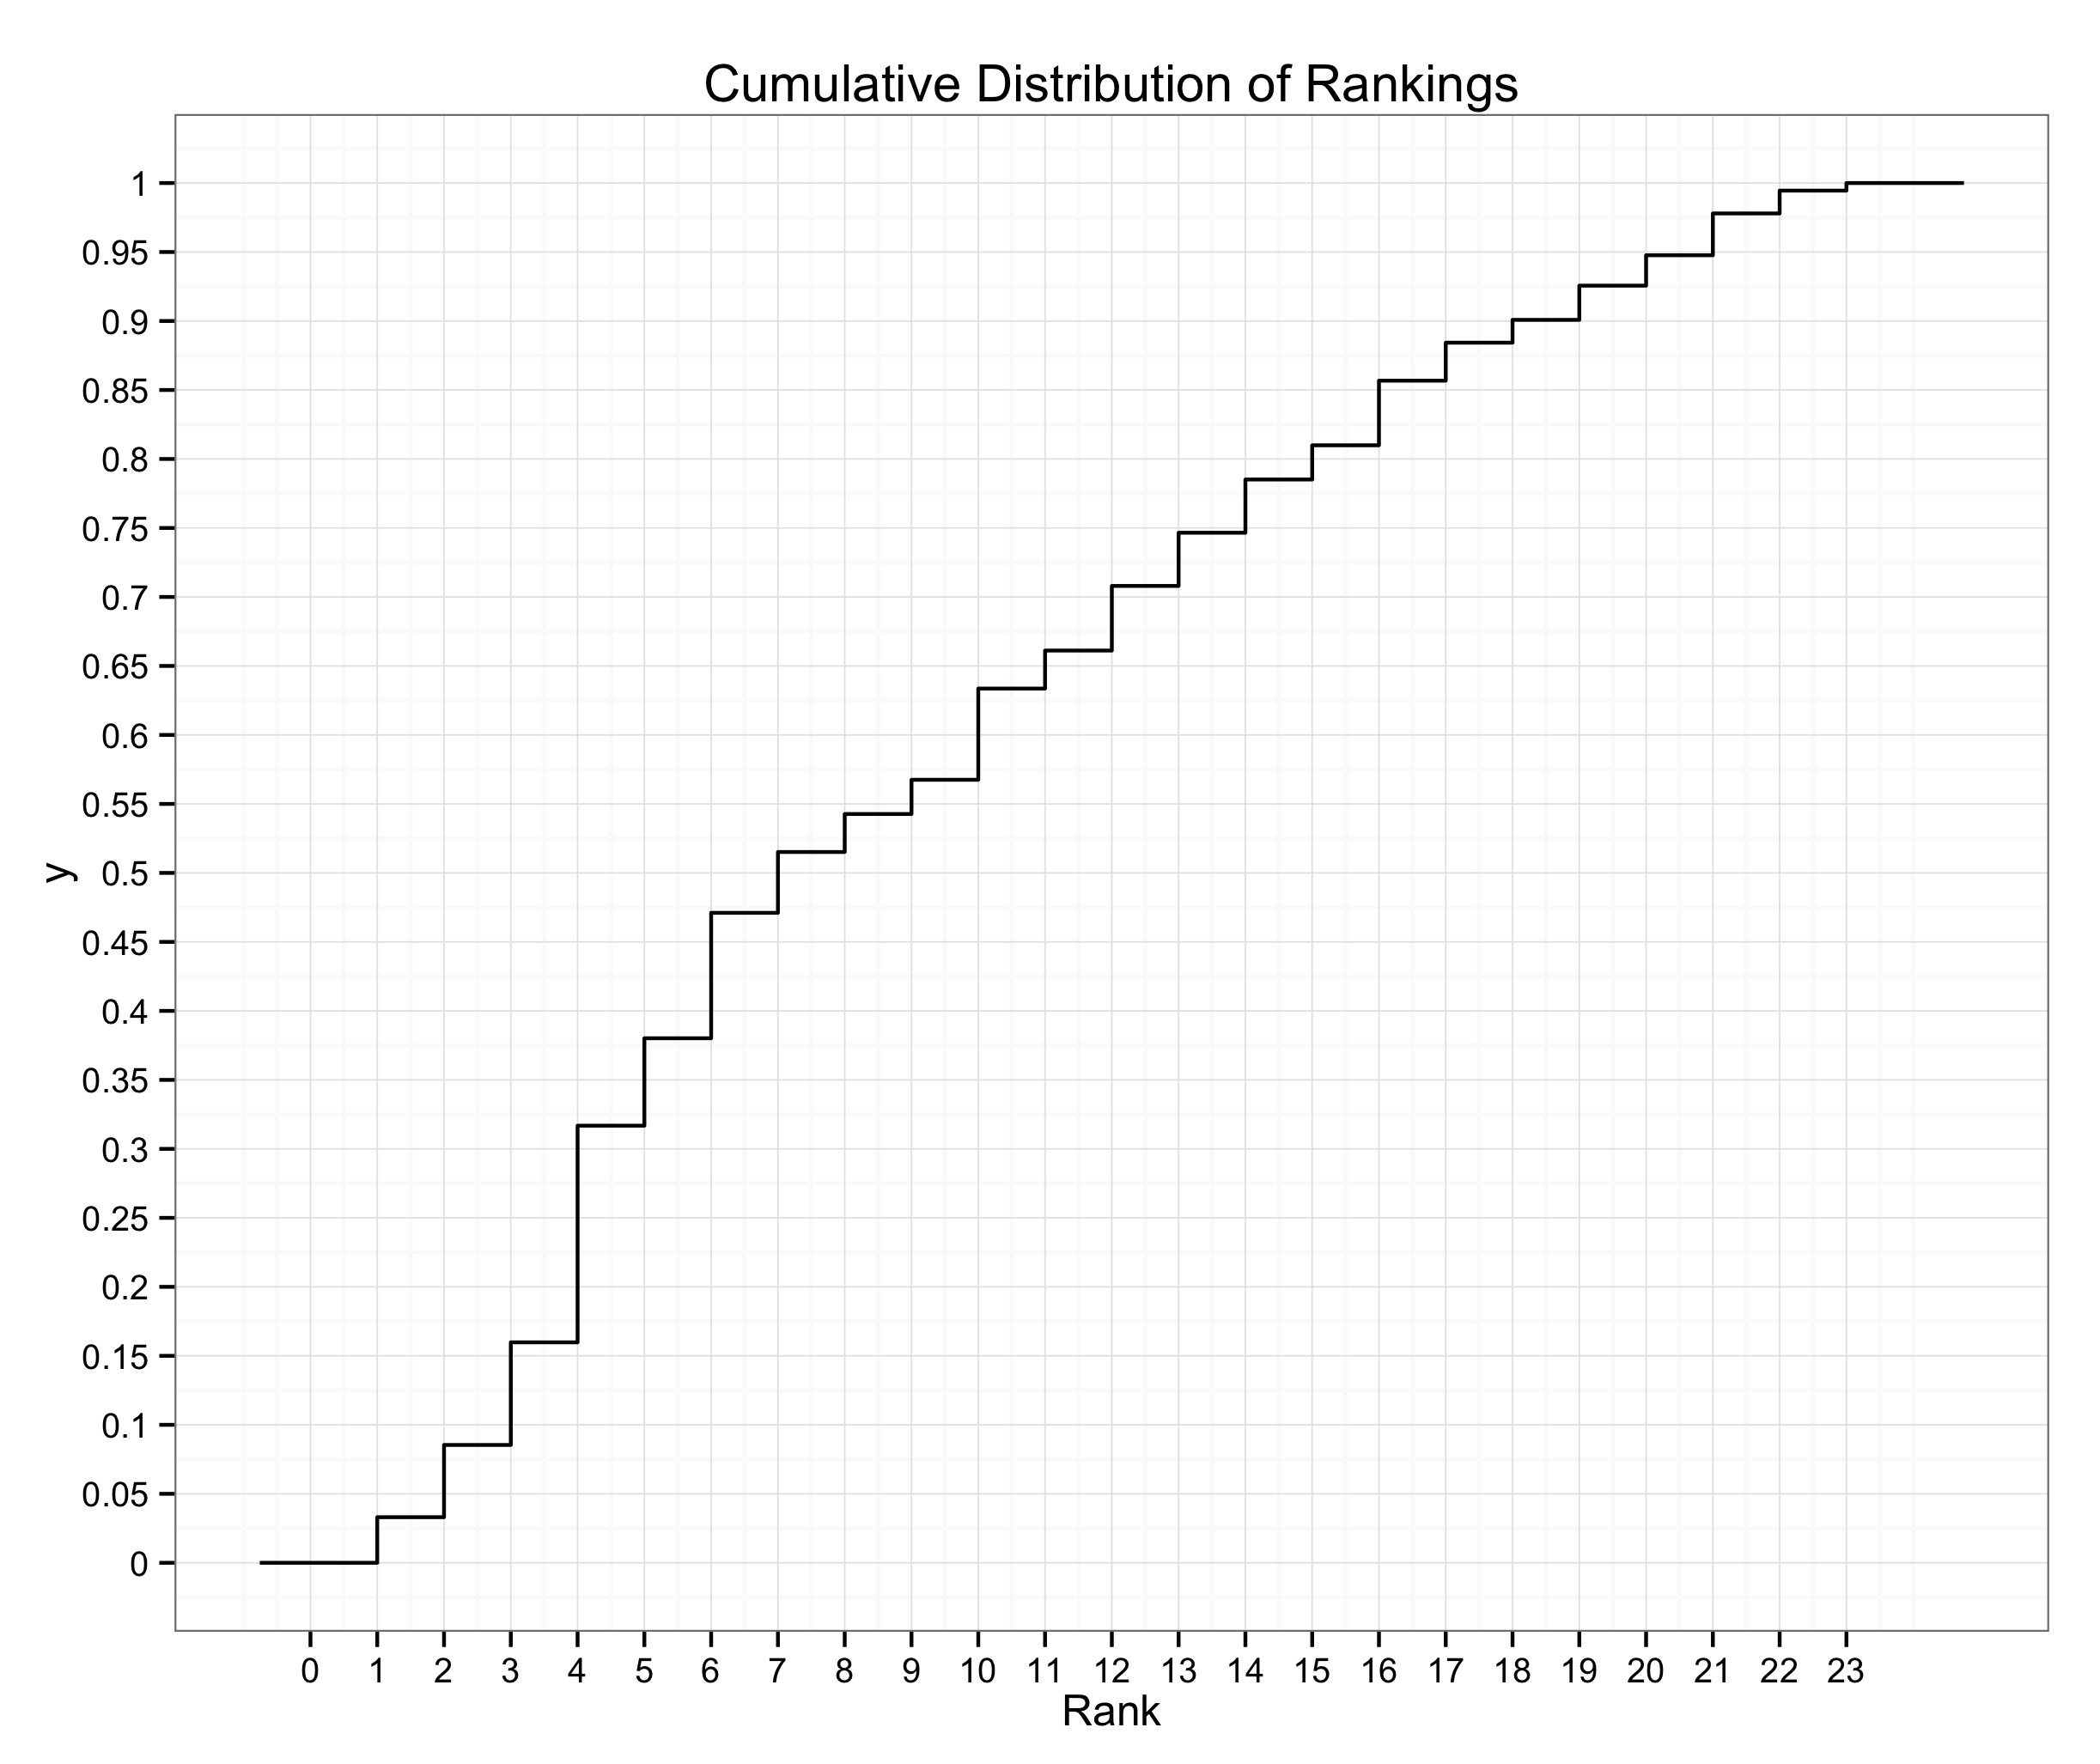
\includegraphics[scale=0.1]{/Users/eaalto/Desktop/Latex/Master_Thesis_Report/images/confRanks/confRankCumSum10.png}
\caption{Image to the left showing a histogram over similarity ranks to the seed playlists, for the playlists to which the false positive samples belong. The figure to the right shows the cumulative distribution of rankings. Both figures show performance for 10 trees in the pre-filtering step.}
\end{figure}

\begin{figure}
20 trees
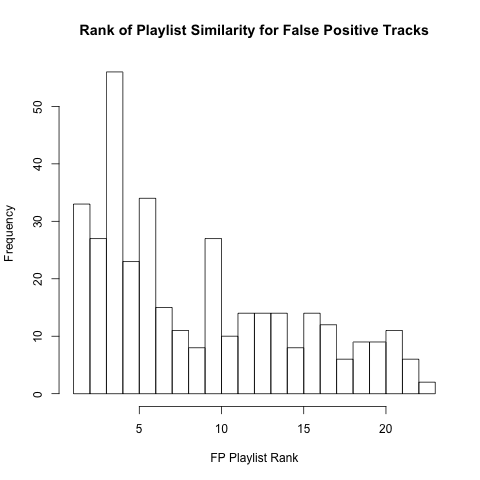
\includegraphics[scale=0.4]{/Users/eaalto/Desktop/Latex/Master_Thesis_Report/images/confRanks/confRankPlot20.png}
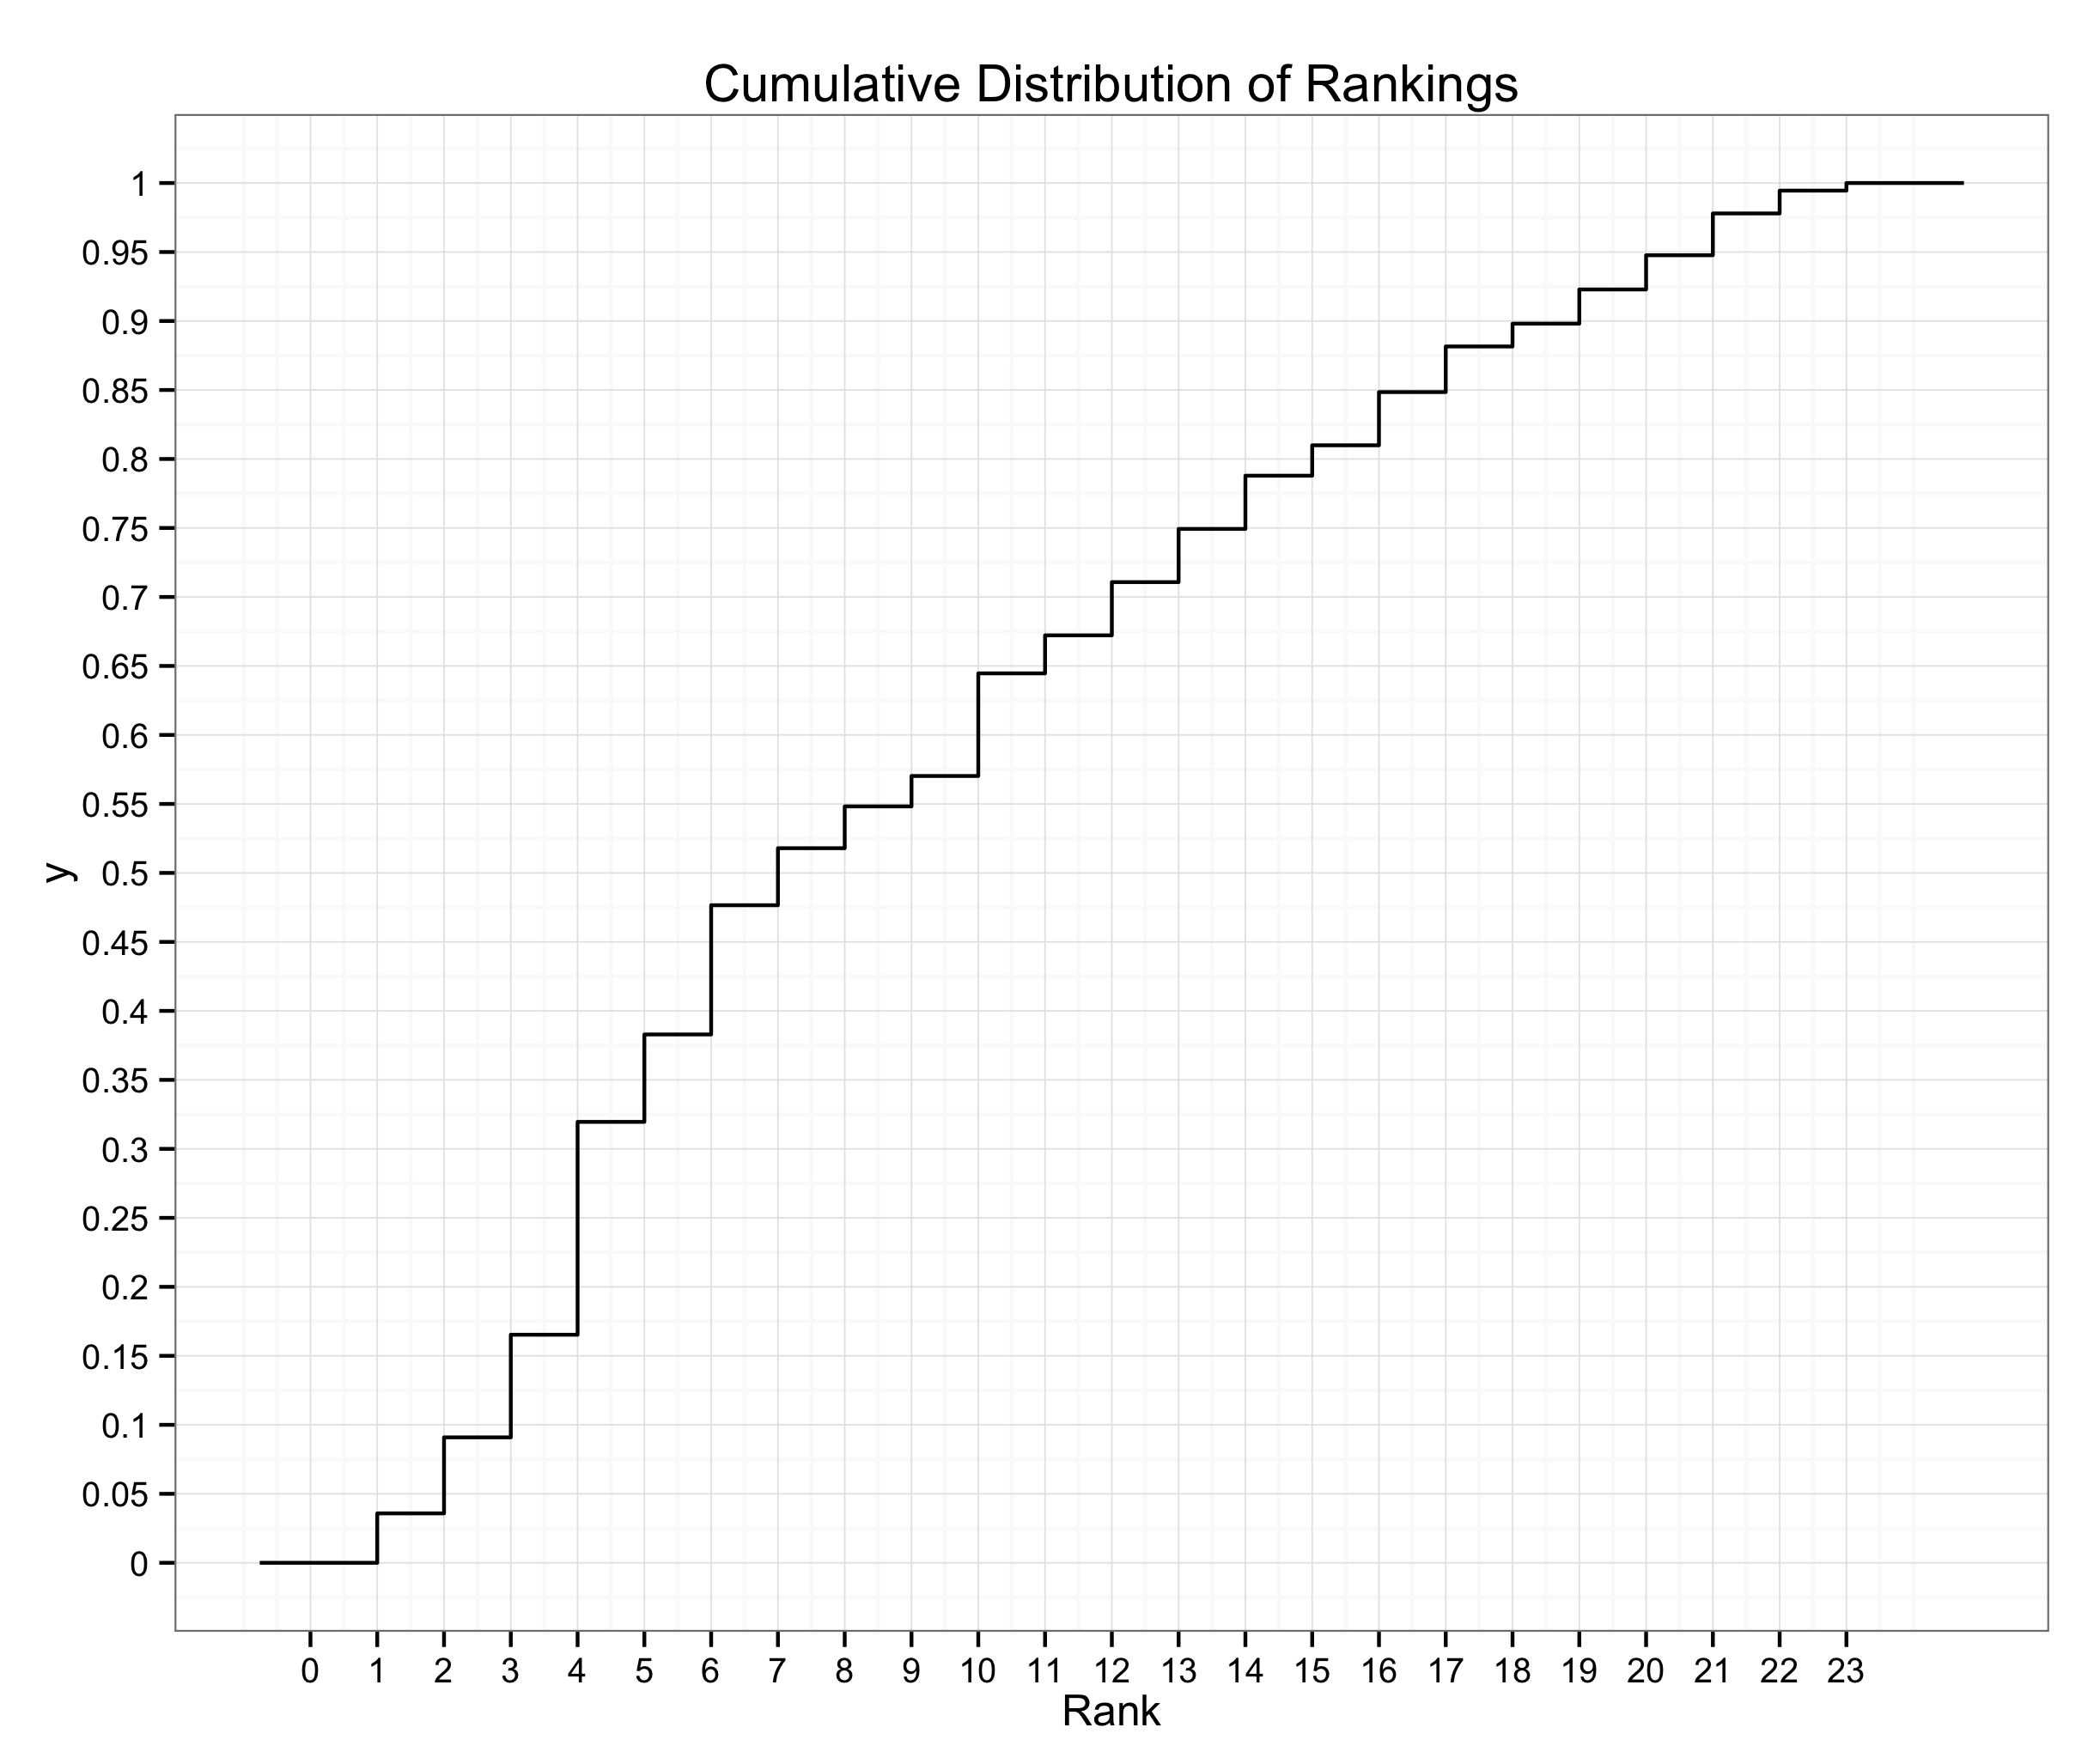
\includegraphics[scale=0.1]{/Users/eaalto/Desktop/Latex/Master_Thesis_Report/images/confRanks/confRankCumSum20.png}
\caption{Image to the left showing a histogram over similarity ranks to the seed playlists, for the playlists to which the false positive samples belong. The figure to the right shows the cumulative distribution of rankings. Both figures show performance for 20 trees in the pre-filtering step.}
\end{figure}

\begin{figure}
30 trees
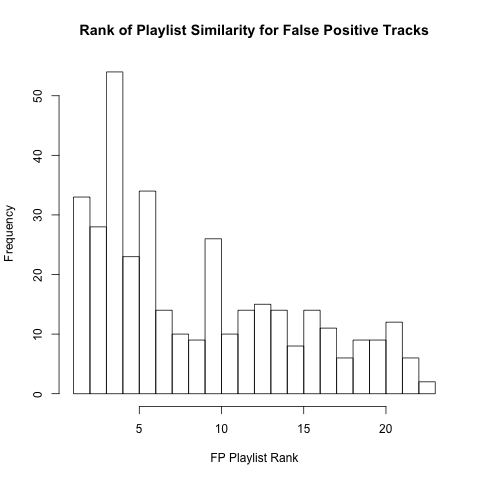
\includegraphics[scale=0.4]{/Users/eaalto/Desktop/Latex/Master_Thesis_Report/images/confRanks/confRankPlot30.png}
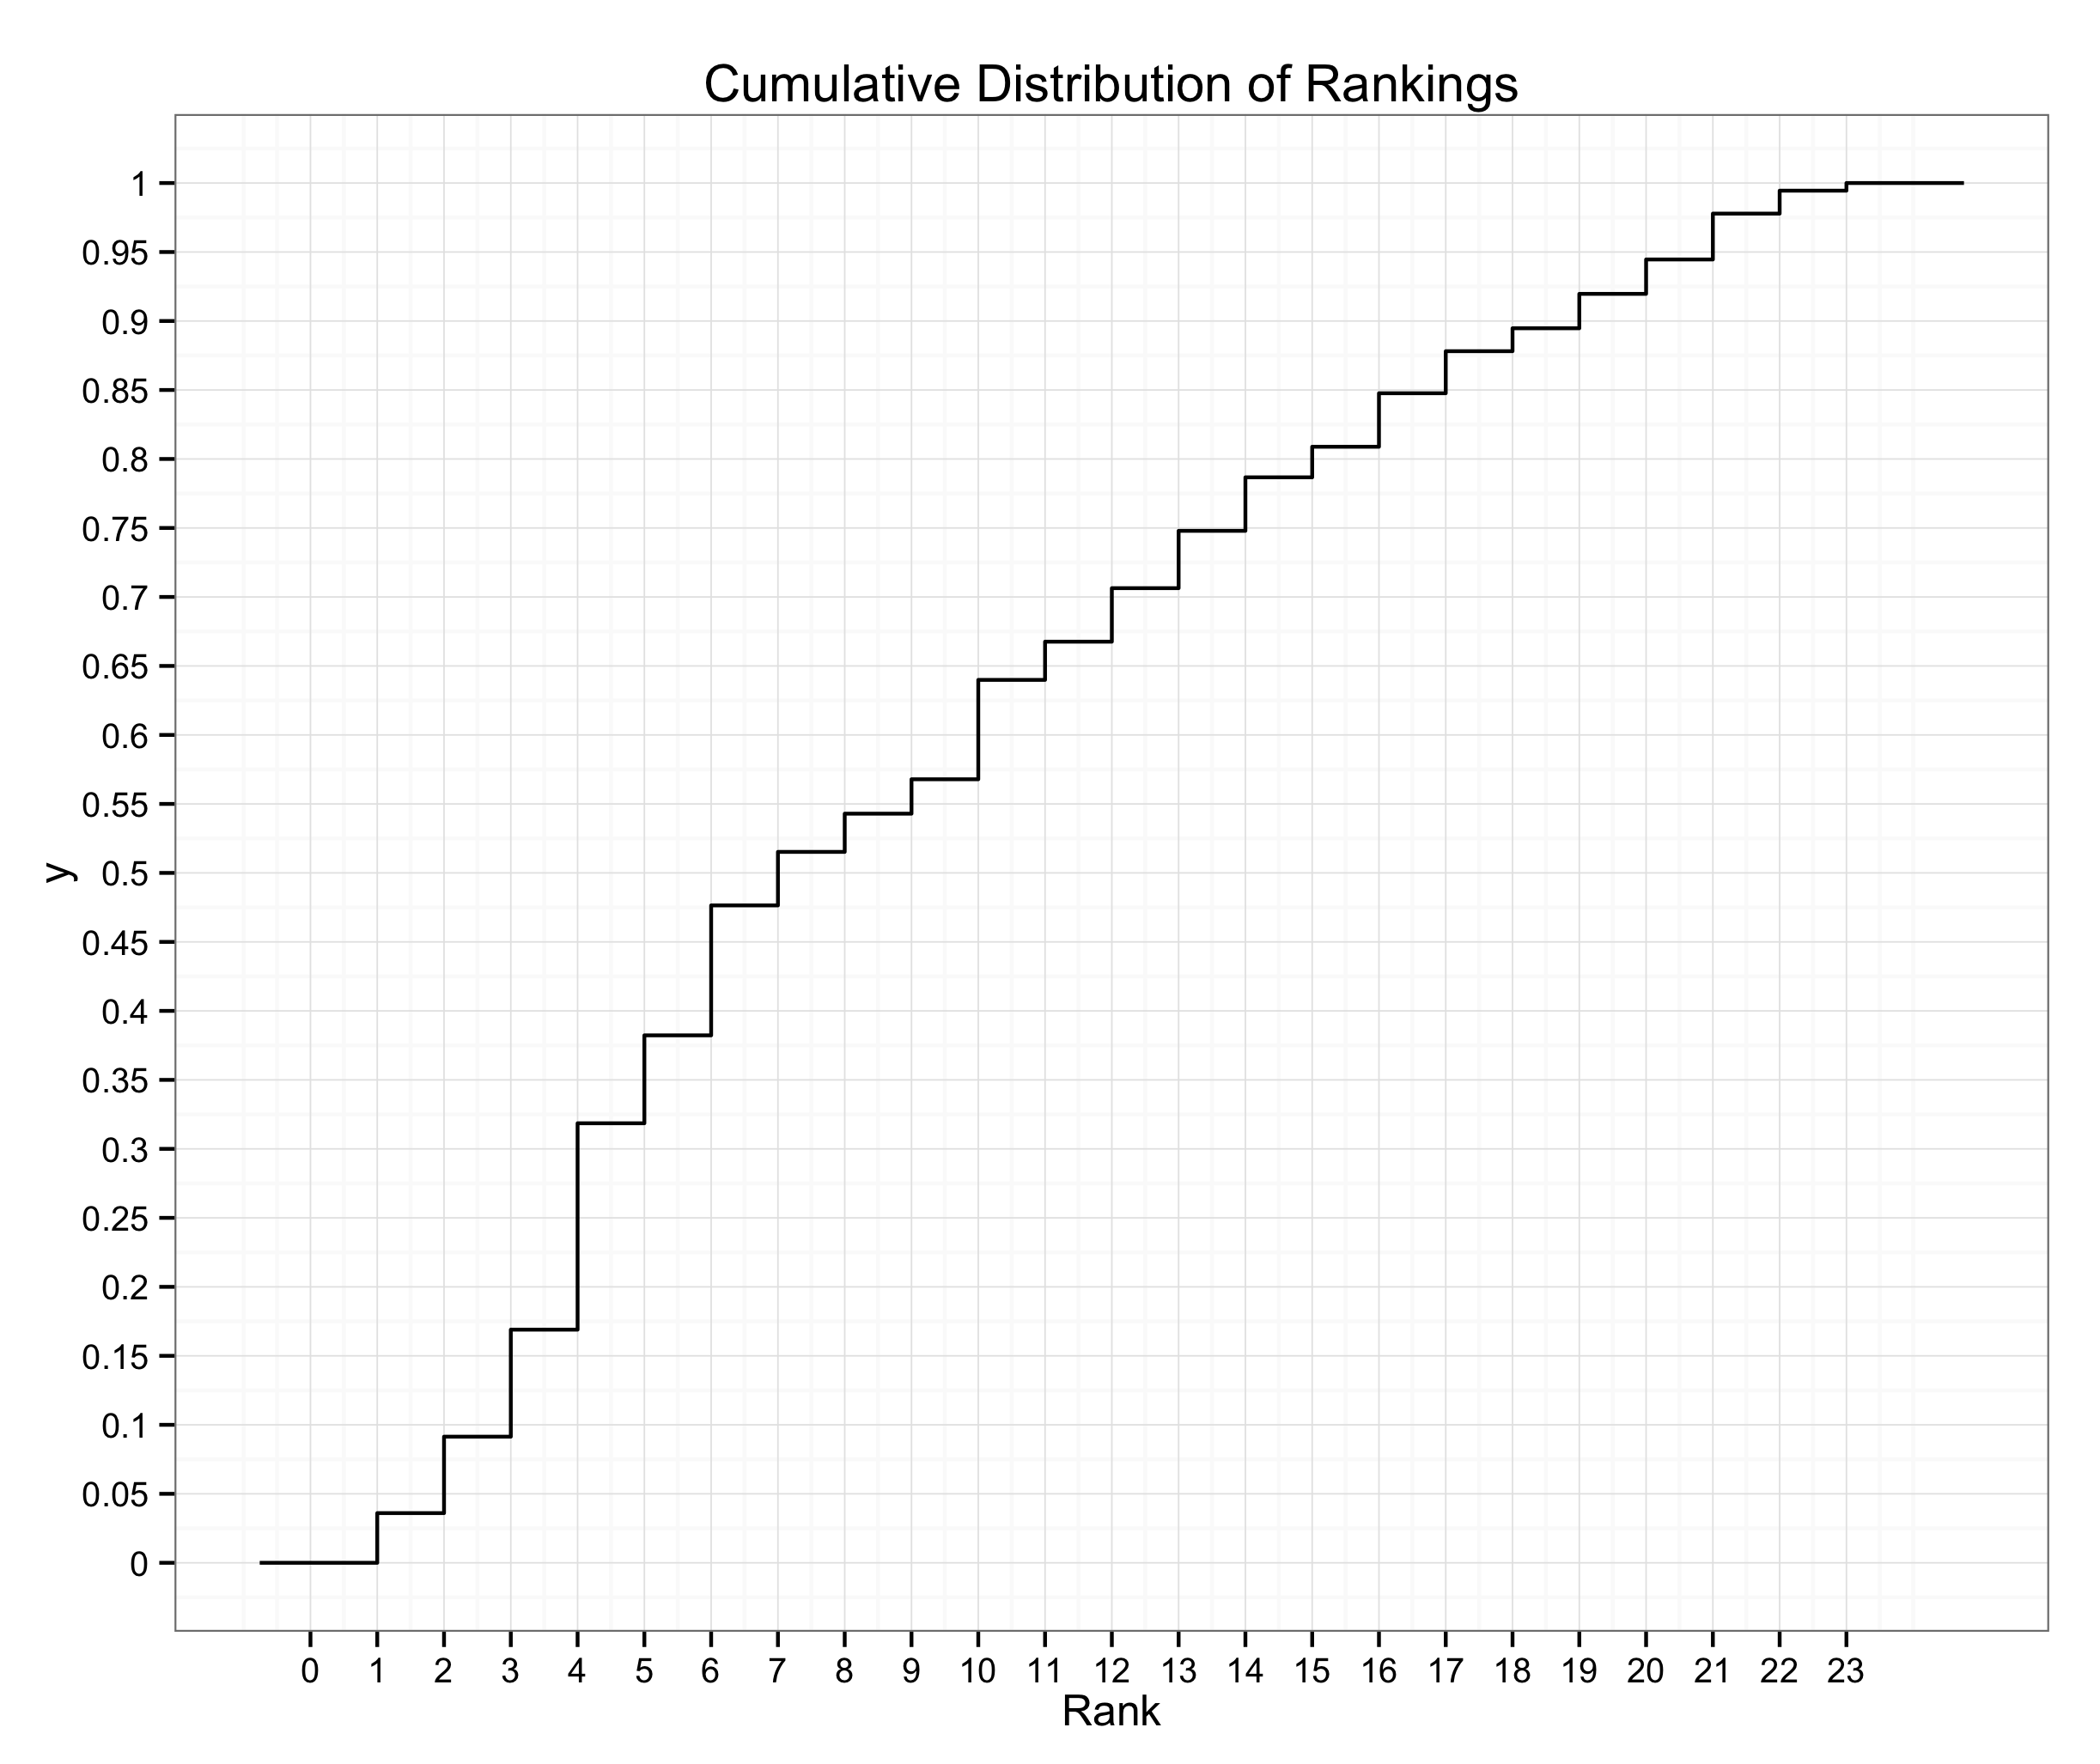
\includegraphics[scale=0.1]{/Users/eaalto/Desktop/Latex/Master_Thesis_Report/images/confRanks/confRankCumSum30.png}
\caption{Image to the left showing a histogram over similarity ranks to the seed playlists, for the playlists to which the false positive samples belong. The figure to the right shows the cumulative distribution of rankings. Both figures show performance for 30 trees in the pre-filtering step.}
\end{figure}

\begin{figure}
50 trees
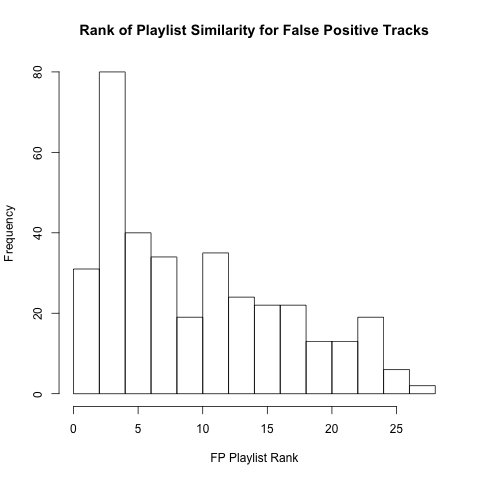
\includegraphics[scale=0.4]{/Users/eaalto/Desktop/Latex/Master_Thesis_Report/images/confRanks/confRankPlot50.png}
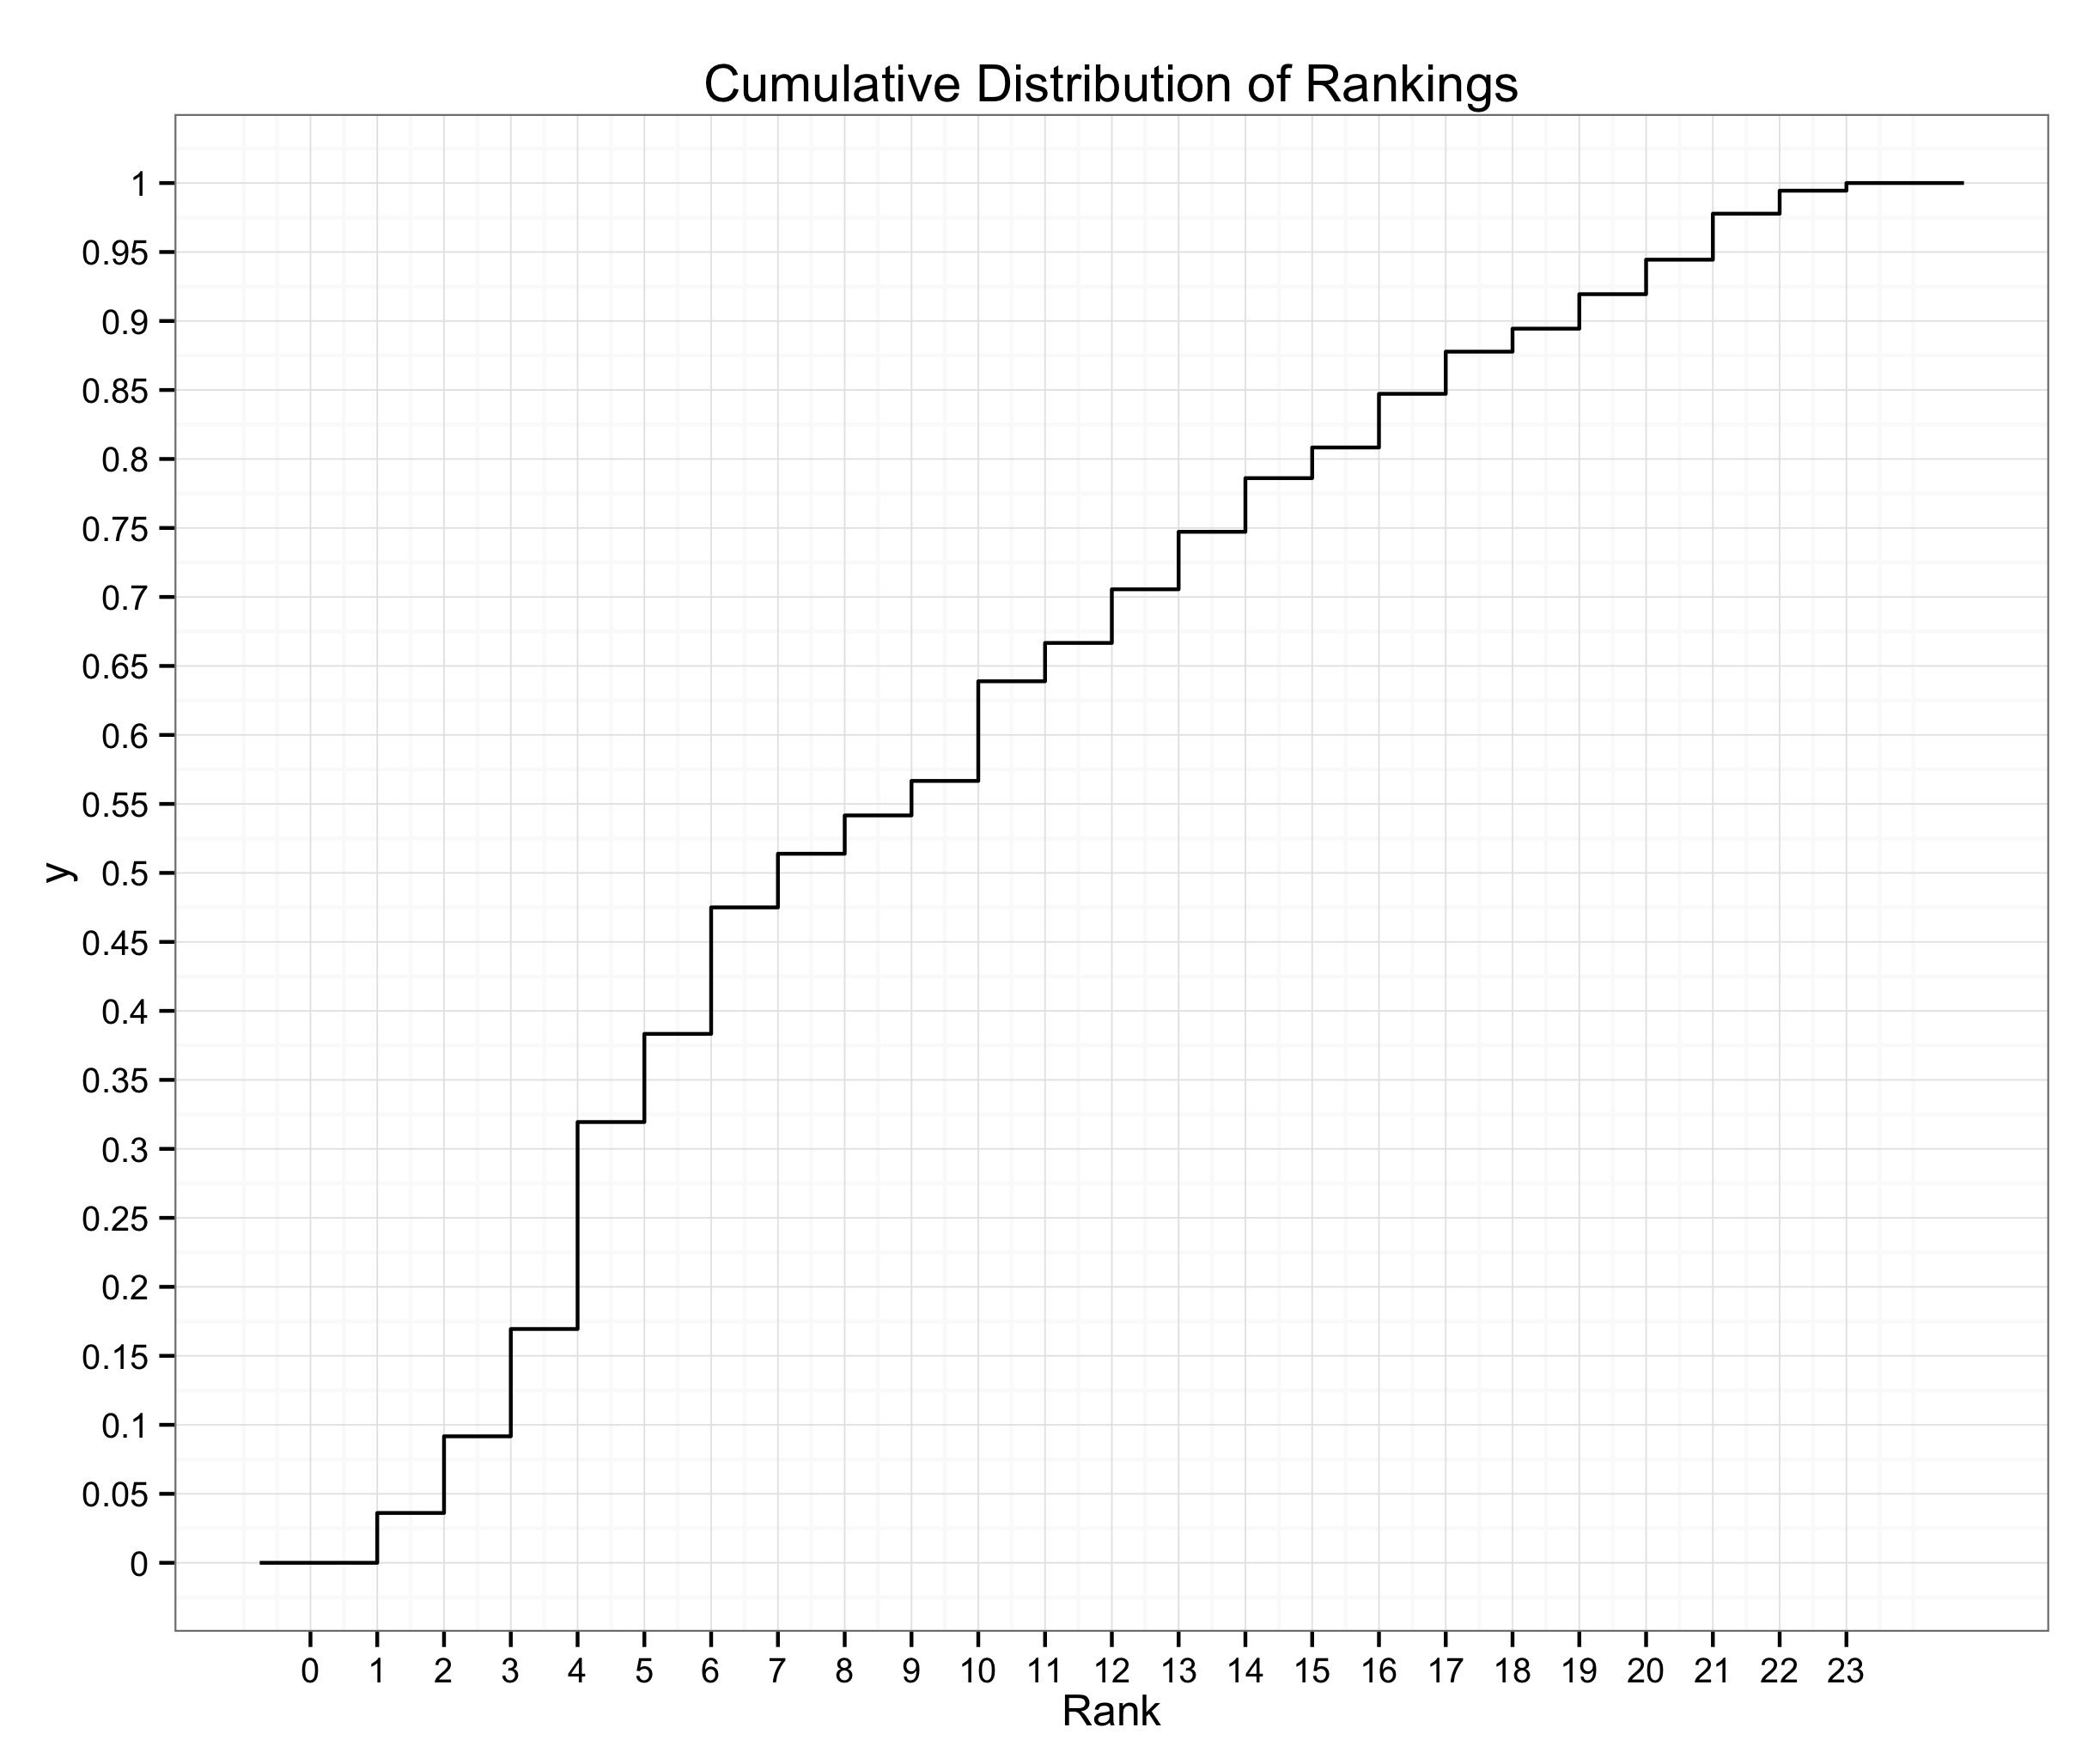
\includegraphics[scale=0.1]{/Users/eaalto/Desktop/Latex/Master_Thesis_Report/images/confRanks/confRankCumSum50.png}
\caption{Image to the left showing a histogram over similarity ranks to the seed playlists, for the playlists to which the false positive samples belong. The figure to the right shows the cumulative distribution of rankings. Both figures show performance for 50 trees in the pre-filtering step.}
\end{figure}

There is a similar behaviour for all number of trees in the approximate nearest neighbour forest where roughly fifty percent of all false positives come from the seven playlists most similar to the seed playlist. This result show that to a high extent tracks regarded as false positives come from playlists that are ranked as being similar to the seed playlist. It is therefore reasonable to believe that precision calculated as tracks coming from playlists in the same cluster is a conservative measure and that the actual results are better than what the precision measure reveals.

\section{Qualitative Evaluations}
To find out if the results from evaluating the rank of playlists from which the confused false positives originated actually means that the tracks selected as candidate songs really are good candidates to a higher extent than what the precision metric reveals and to get an idea of how the selected candidate songs sounded to the human ear qualitative evaluations were performed. Three playlists for which the seed playlists Old School Hip Hop, Old School Rock and Old School Heavy were selected. The reason for selecting these playlists are that they contributed to uniformity of the test as they all were \textit{"Old School"} and all were genre playlists. Also Hip Hop was seen to precision a high performing playlist, Rock middle performing and Metal low performing so to see how well the performance of the quantitative measures responded to listeners opinions. To have a reference point both playlists with songs selected by the model as well as songs from the original curated playlists were selected. To haven an even distribution of biases from the persons listening to the playlists new playlists were created where ten songs in order came from the top ranked candidate songs by the model and the other ten songs, also in order, were the first ones in the seed playlist. Users were then presented with these three playlists and were asked how well the first or last ten songs matched the theme, how many outliers there were and how well the songs matched the theme with outliers removed.

\begin{figure}
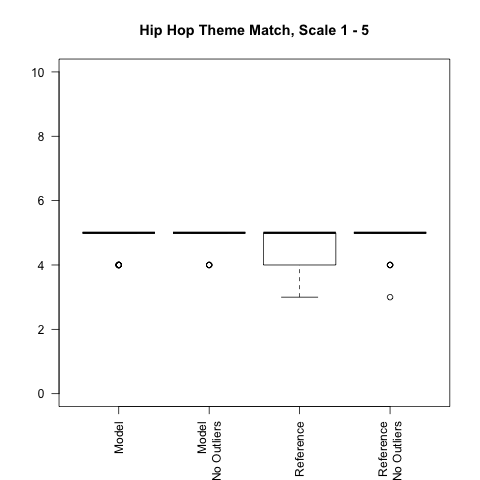
\includegraphics[scale=0.5]{/Users/eaalto/Desktop/Latex/Master_Thesis_Report/images/qvalEvals/hiphop_1_5.png}
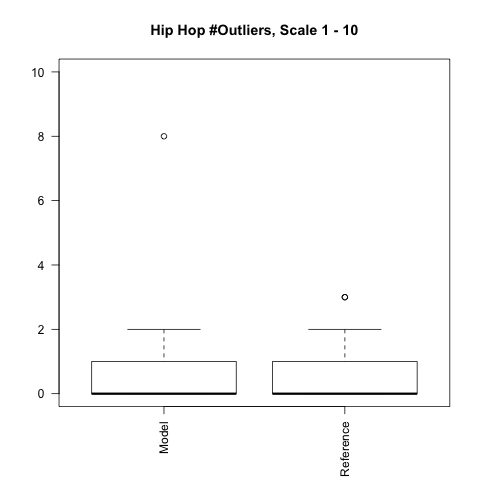
\includegraphics[scale=0.5]{/Users/eaalto/Desktop/Latex/Master_Thesis_Report/images/qvalEvals/hiphop_1_10.png}
\caption{Results from qualitative evaluation for Hip Hop. The image to the left shows the performance of how the tracks in the playlist for qualitative evaluation matches the playlist theme for both the model and the reference playlist. First column shows how well the tracks in the model playlist matches the theme, second column how well the tracks from the model matches the theme with outliers removed. The third and fourth column show the same values for the reference playlist. The image to the right shows the number of outliers found for the playlist from the model or reference respectively. As can be seen the model slightly outperforms the reference. The most probable reason for one person spotting eight outliers in the model is that the user saw one outlier and that was track number eight. Feedback after the qualitative evaluation confirms this.}
\end{figure}

\begin{figure}
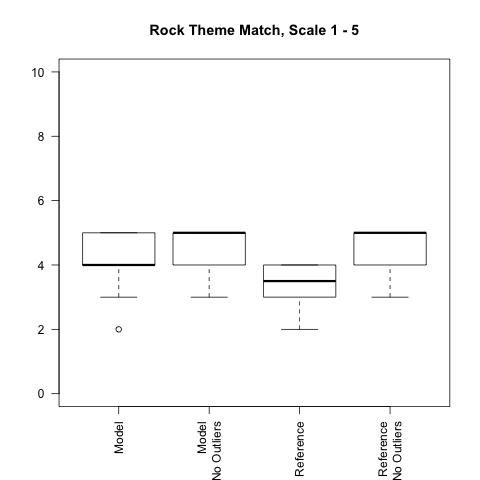
\includegraphics[scale=0.5]{/Users/eaalto/Desktop/Latex/Master_Thesis_Report/images/qvalEvals/rock_1_5.png}
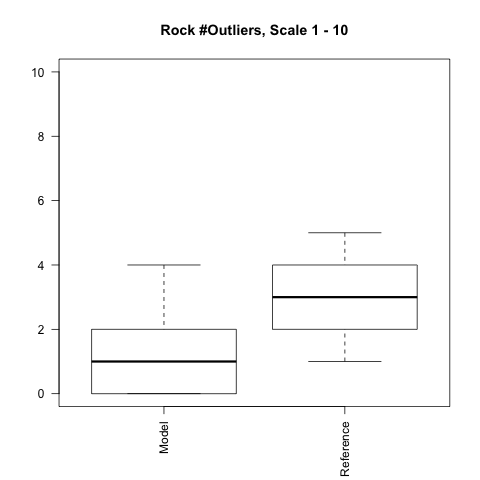
\includegraphics[scale=0.5]{/Users/eaalto/Desktop/Latex/Master_Thesis_Report/images/qvalEvals/rock_1_10.png}
\caption{Results from qualitative evaluation for Rock. The image to the left shows the performance of how the tracks in the playlist for qualitative evaluation matches the playlist theme for both the model and the reference playlist. First column shows how well the tracks in the model playlist matches the theme, second column how well the tracks from the model matches the theme with outliers removed. The third and fourth column show the same values for the reference playlist. The image to the right shows the number of outliers found for the playlist from the model or reference respectively. As can be seen the model outperforms the reference. A reasonable explanation to the low performance of the reference could be that experts designing the playlist and the users evaluating the playlist have different opinions about what rock is. Is the song \textit{Son of a preacher man} that was present among the reference songs old school rock or pop for example.}
\end{figure}

\begin{figure}
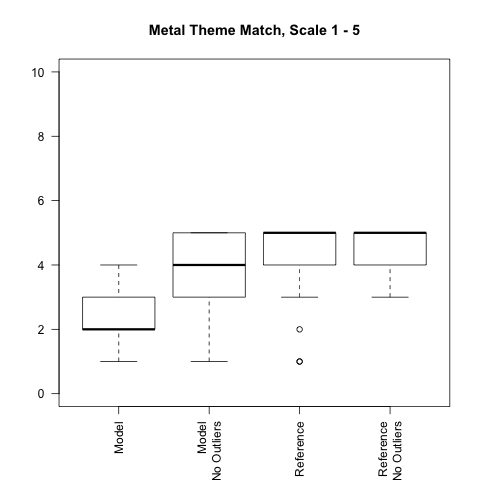
\includegraphics[scale=0.5]{/Users/eaalto/Desktop/Latex/Master_Thesis_Report/images/qvalEvals/metal_1_5.png}
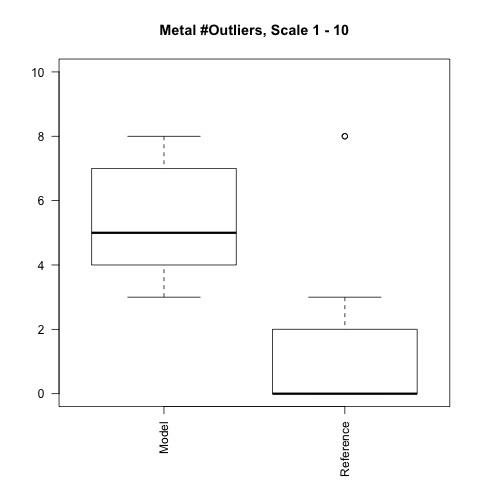
\includegraphics[scale=0.5]{/Users/eaalto/Desktop/Latex/Master_Thesis_Report/images/qvalEvals/metal_1_10.png}

\caption{Qualitative results for the Metal playlists. The image to the left shows the performance of how the tracks in the playlist for qualitative evaluation matches the playlist theme for both the model and the reference playlist. First column shows how well the tracks in the model playlist matches the theme, second column how well the tracks from the model matches the theme with outliers removed. The third and fourth column show the same values for the reference playlist. The image to the right shows the number of outliers found for the playlist from the model or reference respectively. As can be seen the reference clearly outperforms the model. As one user misunderstood the outlier scale for Hip Hop it is reasonable to assume that the one person ranking the number of outliers for the metal playlist having commited the same mistake, but as opinions about music differ we cannot be sure about this.}
\end{figure}

As can be seen form the user evaluations surprisingly the tracks from the model were ranked higher than those taken from the curated playlists for both Hip Hop and Rock. The model selected tracks for metal were ranked lower, but the users rankings confirmed the notion that precision as used for the quantitative evaluations was a conservative measure as users found less outliers than there were false positives from the quantitative evaluation.

\chapter{Discussion and Future Work}

\section{Discussion}
Using playlists is an attractive means of consuming music. This can be shown by the fact that in the Spotify music library the number of songs is in magnitude of millions but the number of playlists is in magnitude of billions. It is therefore desirable for a music provider to be able to automatically generate playlists adapted to a users distinct taste. One way of doing this is to generate playlists from an initial seed playlist which the user can specify.
 The method used in this thesis provides a scalable and parallelizable approach for a step on the way of creating automatically generated playlists of high quality, merely the selection of candidate songs for a generated playlist. The method has proven to perform better than a baseline in form of random sampling from approximate nearest neighbours for candidate song selection. The baseline might seem trivial at a glance, but these results imply that learning a playlist representation present a superior approach for playlist song selection than neighbourhood-based approaches. Results therefore confirm that the initial assumption of regarding a playlist as a good mix of songs and therefore regarding variance as a important factor to distinguish playlist characteristics is a valid approach.
 Quantitative results also imply that the actual quality of songs selected for playlist generation is better than the one measured by calculating precision. Qualitative assesments further strengthens this hypothesis. The qualitative assesments made ranked the generated playlists higher than the ones from where the representation was learned in two out of three cases. The third cased consisted of a playlist with the second lowest precision in the entire experiment and the evaluations made qualitatively suggest a more than a hundred percent higher actual precision of that playlist than what the precision measure entails. These results together suggest that learning a playlist representation in an eigenbased way is an effective approach for playlist generation together with approximate nearest neighbour pre-filtering. Lastly, as rankings of false positives for the precision measure to a high extent came from similar playlists it is also reasonable to assume that the performance of the model would be even better should a bigger data set with more relevant tracks for each seed playlist be present. 

\subsection{Complexity Analysis}
One reason to why time complexity is important in the field of Machine Learning is that it gives a unified measure of the time and resources needed to solve a problem. One example is if the run-time for an algorithm is asked a not uncommon answer is that it takes x time. An answer as such gives no information of how the algorithm scales, whether it is implemented in an efficient manner or not or if the run-time is hardware dependent. For example, an algorithm that take one day to solve a problem, but has linear time complexity can solve the same problem for the double amount of data in two days. For an algorithm with quadratic running time it would take four days to solve the same problem should input data be doubled. Another example is if an algorithm is run on a brand new computer or a computer that is 15 years old, simply stating the run-time does not give a unified measure as run time will change depending on hardware. Lastly, given the size of input data and the time complexity of the algorithm a hint of the expected run-time can be obtained and used for debugging purposes.
 As can be easily understood analyzing time complexity within the machine learning field is essential to understand the scalability of a machine learning algorithm. An algorithm that grows faster than linear with data quickly becomes unfeasible as the amount of data used grows large. In the case of Spotify the number of tracks in the song library and the number of users are in the magnitude of millions or tens of millions which means that even a linear run-time might be too slow to be practically usable.
 
Computational complexity theory is about analyzing the amount of resources needed to solve a particular problem and classifying problems according to how difficult they are to solve. Resources needed to solve a problem generally mean running time or memory, but could also include randomness or communication. 

Analyzing the time it takes for an algorithm to solve a problem is also called time complexity. Time complexity is a quantification of the time needed to solve a problem as a function of the length or size of the input. A common way to describe time complexity is the asymptotic behaviour of running time needed as a function of input, also called \textit{Big-O} notation. Time complexity analysis with \textit{Big-O} notation takes the dominant terms into regard as input data grows towards infinity. For example if we have a problem that for the length of input \textit{n} requires $(2n)^2$ operations the problem has a time complexity of $O(n^2)$. \textit{Big-O} notation assumes that some operations called trivial operations take a constant time to perform, \textit{O(1)}, and if \textit{n} such operations are performed the time complexity becomes \textit{O(n)}. All operations that do not grow with the size of input data are dropped using \textit{Big-O} notation. For example if an algorithm needs a cubic number of operations for each input data term and an additional thousand operations that do not change with the size of input data the total amount of operations needed is $n^3 + 1000$ which becomes $O(n^3)$

The first step in the model is to create a covariance matrix from the features of tracks in the seed playlist. The computational complexity of creating a covariance matrix is $O(ND^2)$ where \textit{N} is the number of tracks in the playlist and \textit{D} is the number of features that represent each track\cite{kwatra2010fast}. Once the covariance matrix is created an eigen value decomposition is needed to get an orthogonal representation of features in the data, the time complexity for the eigen value decomposition is in the magnitude of $O(D^3)$ where \textit{D} is the number of rows, or columns due to symmetry, in the covariance matrix which is equal to the number of dimensions of features for each playlist track\cite{pan1999complexity}. After the eigendecomposition a projection matrix is needed to project tracks into the principal component space of a seed playlist. To create the projection matrix one matrix inversion with complexity of $O(D^3)$ and three matrix multiplications, also with time complexity of $O(D^3)$ are needed, with a resulting time complexity of creating the projection matrix of $O(D^3)$. To project each track into the principal component space a matrix vector multiplication is needed with time complexity of $O(D^2)$ and this is done for each track which yields a resulting time complexity of $O(ND^2)$ where \textit{N} are the number of tracks to be projected. The calculation of relative change in magnitude requires calculating the length of each track represented as a vector which includes a squared root operation and thus has the time complexity of $O(D^2)$. Creating a covariance matrix, eigendecompose it and creating a projection matrix does only have to be done once and as the number of tracks in a playlist does not exceed the magnitude of hundreds and the number of dimensions for each track is fixed the steps of the model before projecting tracks can be regarded as constant operations. Using approximate nearest neighbours for one track is a constant time operation and needs to be done for each track in the seed playlist which gives a resulting time complexity of \textit{O(N)} where \textit{N} is the number of tracks in the seed playlist. The resulting complexity of the model thus becomes $O(nD^2)$ where \textit{n} are the number of tracks obtained by using approximate nearest neighbours and \textit{n << N} where \textit{N} is the total number of tracks in the music library. This yields a resulting time complexity which is sublinear in the number of tracks and quadratic in the number of features. What is further interesting is that the projection of tracks into subspaces can be done in parallel. 
 
\section{Future Work}
\textit{So many things to do and so little time} \\The Joker\\\\
A given first step of continuing the work presented in this thesis would be to also take the ordering of songs, once selected as good candidate for playlist generation, into consideration. It would also be interesting to study how the amount of variance captured when creating a principal component space for a playlist would relate to the quality of the songs selected. Feature selection has been outside the scope of this thesis, but it is very likely that the creation of better features would make the model perform better. One particularly interesting feature that has been lacking for this thesis is time, which is an important factor in the music context. The use of a larger data set for better evaluation is also of interest as this would give a better generalizability than what could be fitted into the scope of this thesis. Lastly, and what seems like the most fun, would be to consider other covariance functions than the linear one and to use a model, such as probabilistic principal component analysis, which apart from covariance also can take location, such as in the form of the mean, into consideration intrinsically.
\bibliography{refList}
\bibliographystyle{plain}

\appendix
\addappheadtotoc
\chapter{RDF}\label{appA}

\begin{figure}[ht]
\begin{center}
And here is a figure
\caption{\small{Several statements describing the same resource.}}\label{RDF_4}
\end{center}
\end{figure}

that we refer to here: \ref{RDF_4}
\end{document}
